\chapter{Молекулярно-динамическое моделирование процессов роста и диссоциации гидрата метана}
\section{Затвердевание переохлажденной двухфазной системы метан-вода}
Нами было произведено моделирование процесса зародышеобразования и роста гидрата метана при температуре $T=210$К и давлении $p=500$ атмосфер, выполненное с различными скоростями охлаждения. Начальная конфигурация системы представляла собой 64 ($4\times 4\times 4)$ элементарные ячейки $sI$-гидрата метана, состоящая из 2944 молекул воды и 512 молекул метана (рис. \ref{fig3.1} и рис. \ref{fig3.2}). Длина ребра кубической ячейки моделирования составляла $\approx 50$ нм. В качестве используемой модели межчастичного взаимодействия была выбрана крупнозернистая модель гидрата метана, упомянутая ранее в данной работе. Информация о начальных положениях частиц была получена из работы[41], причем молекулы воды помещались в позициях атомов кислорода, а молекулы метана располагались в центрах полостей кристаллической решетки. Моделирование производилось в $NPT$-ансамбле с использованием термостата и баростата Нозе-Гувера. Интегрирование уравнений движения производилось в программном пакете моделирования классической молекулярной динамики LAMMPS[42] с использованием скоростного алгоритма Верле. Временной шаг интегрирования $\tau$ был взят равным 10 фс. Применялись периодические граничные условия для всех стенок ячейки моделирования. Графические изображения ячейки моделирования были отрисованы в программном обеспечении для визуализации и анализа результатов молекулярной динамики OVITO[43].

Причина выбора крупнозернистой модели обоснована её большей вычислительной эффективностью по сравнению со всеатомными моделями, поскольку для получения фазы гидрата из жидкой системы требуется симулировать её на протяжении длительного (вплоть до нескольких микросекунд) промежутка времени, что при использовании более сложных моделей и ограниченности имеющихся в распоряжении вычислительных ресурсов заняло бы достаточно большой (около 100 дней для одного моделирования) срок.

\begin{figure}[H]
    \centering
    \begin{minipage}{\linewidth}
        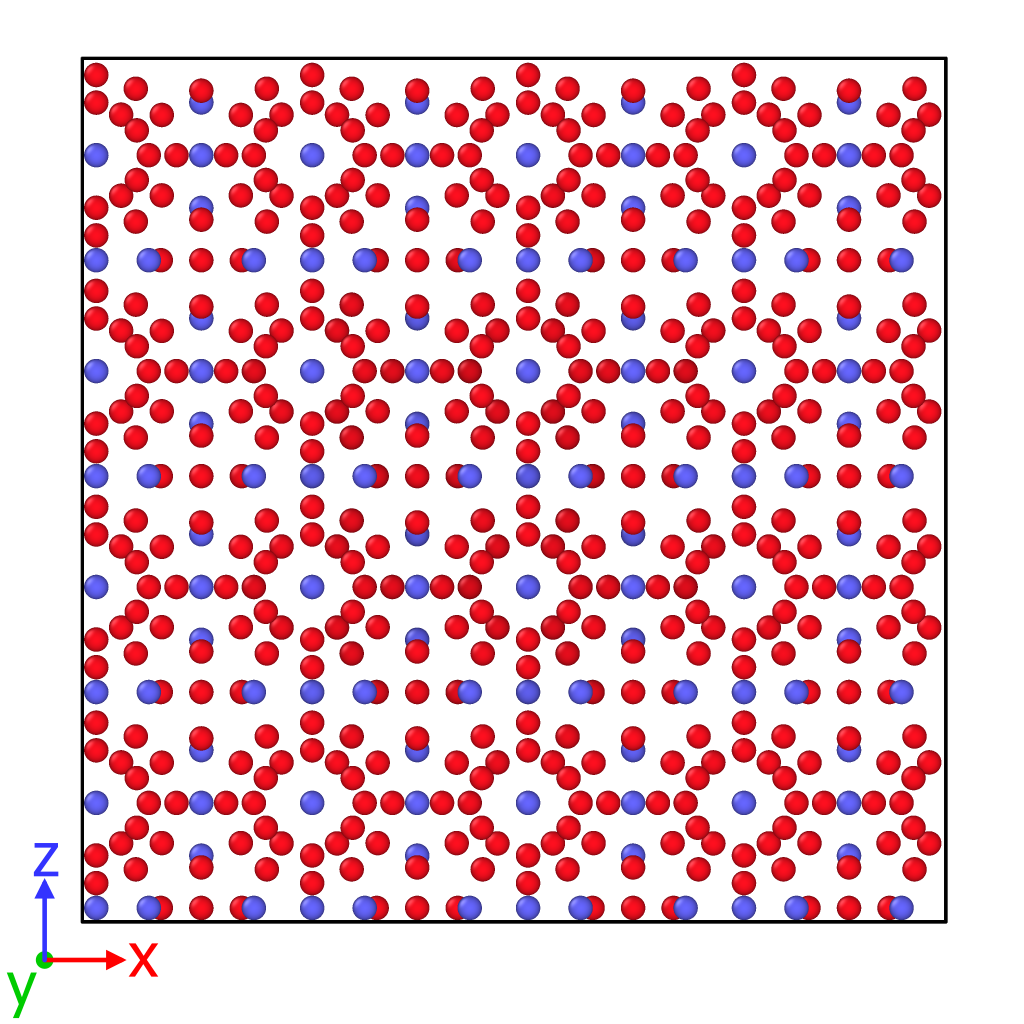
\includegraphics[width=.49\linewidth]{figures/unit1.png}
        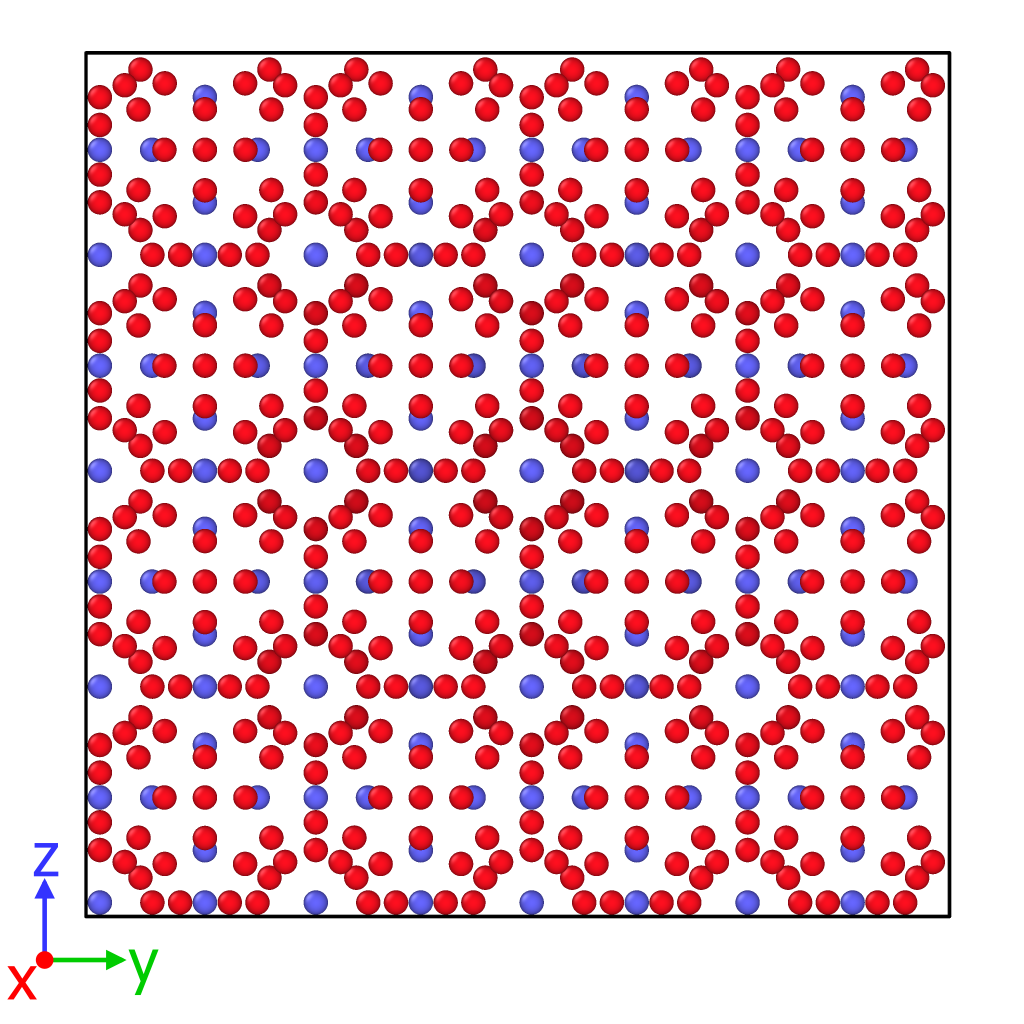
\includegraphics[width=.49\linewidth]{figures/unit2.png}
    \end{minipage}
    \begin{minipage}{\linewidth}
        \centering
        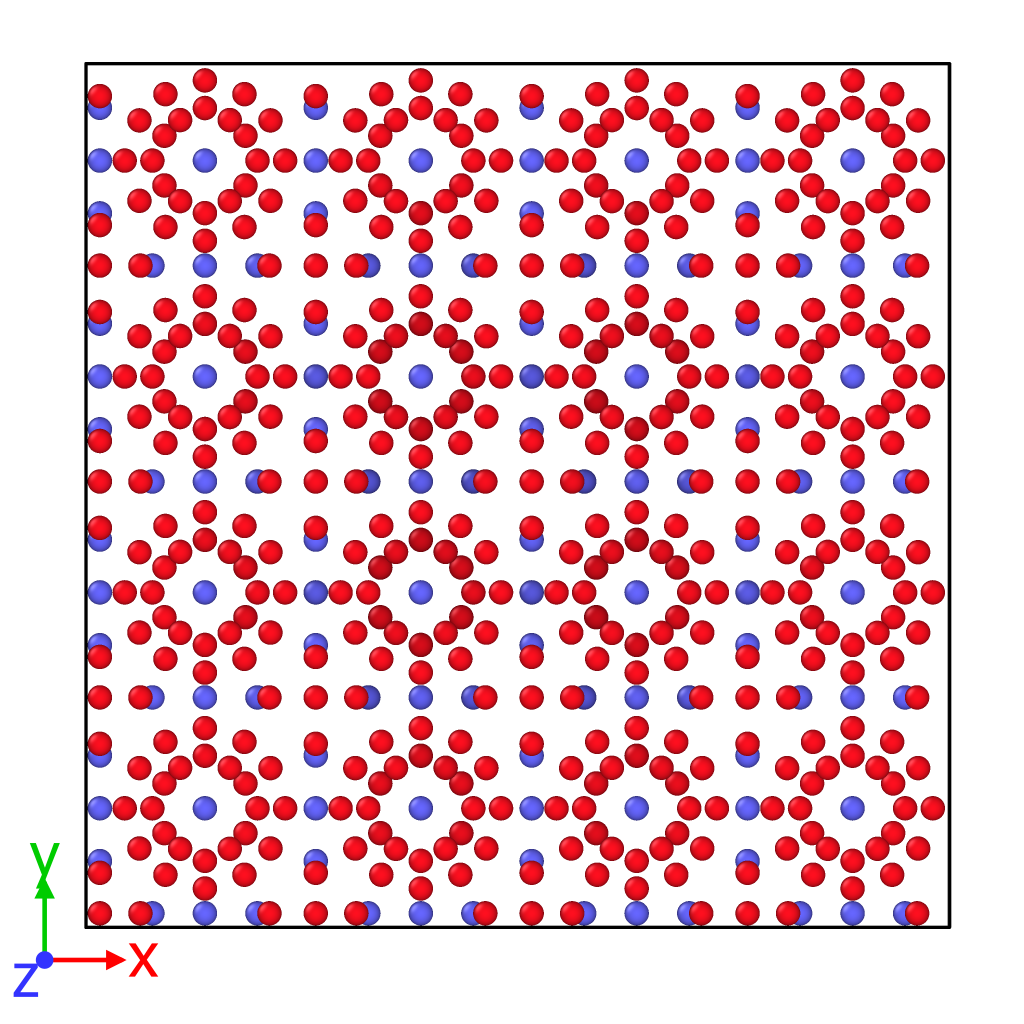
\includegraphics[width=.5\linewidth]{figures/unit3.png}
    \end{minipage}
    \begin{minipage}{\linewidth}

    \end{minipage}
    \caption{Исходная конфигурация ячейки моделирования в трех проекциях. Красными шариками изображены молекулы воды, синими – молекулы метана.}
    \label{fig3.1}
\end{figure}

\begin{figure}[H]
    \centering
    \begin{minipage}{\linewidth}
    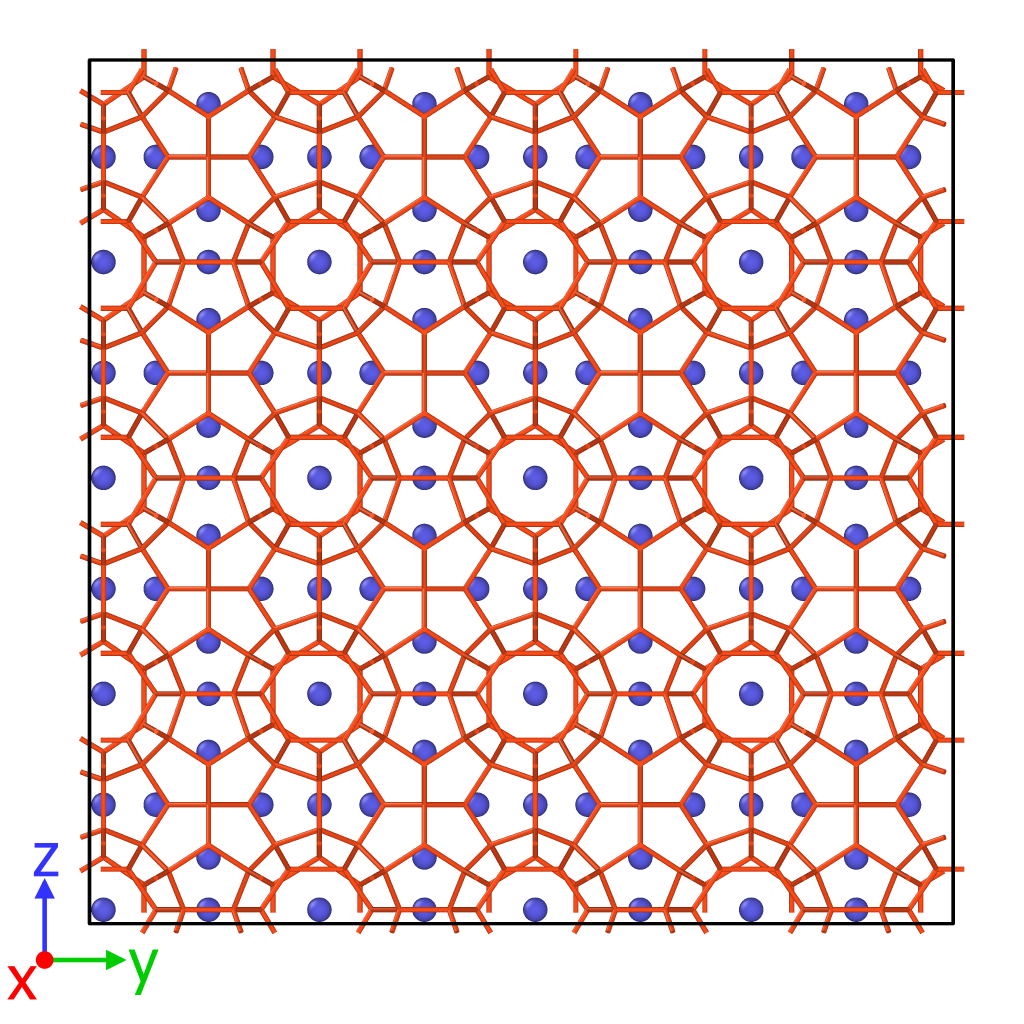
\includegraphics[width=.49\linewidth]{figures/unit1a.png}
    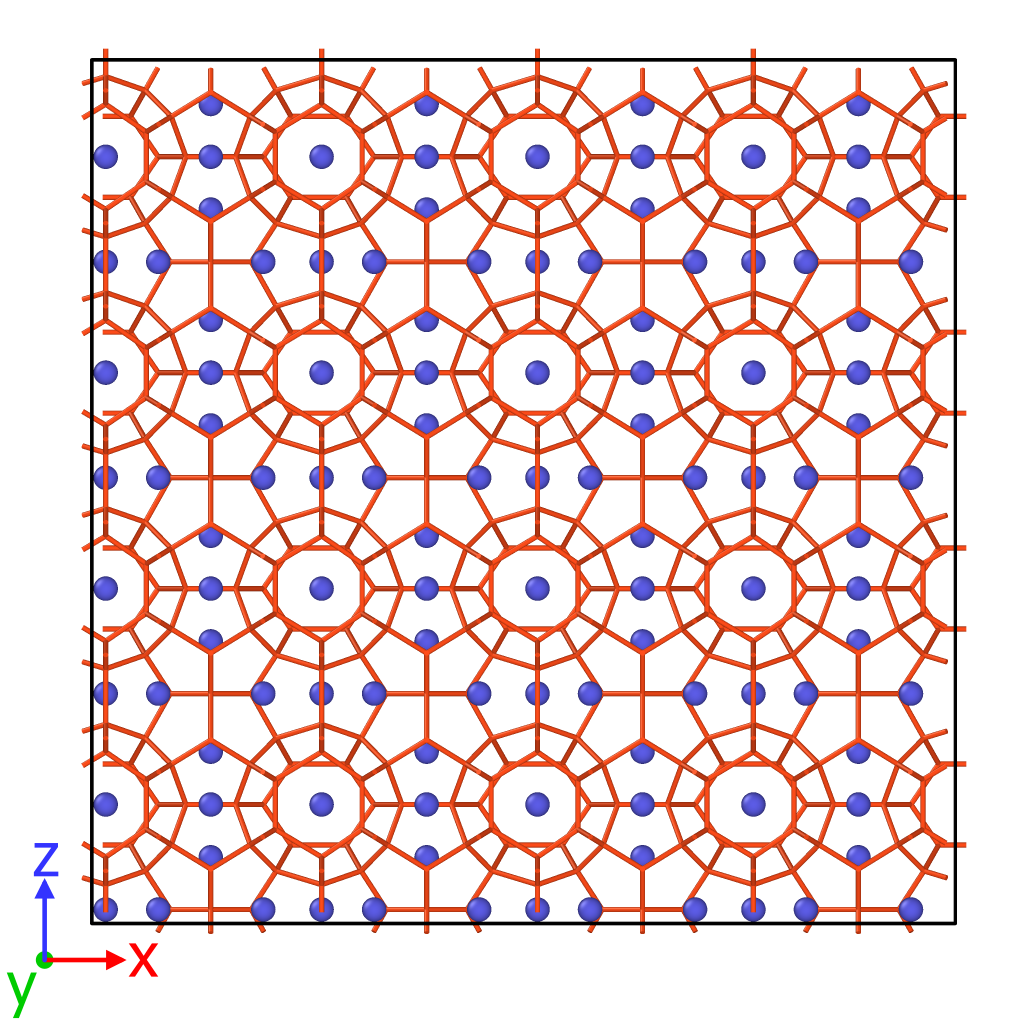
\includegraphics[width=.49\linewidth]{figures/unit2a.png}
    \end{minipage}
    \begin{minipage}{\linewidth}
        \centering
        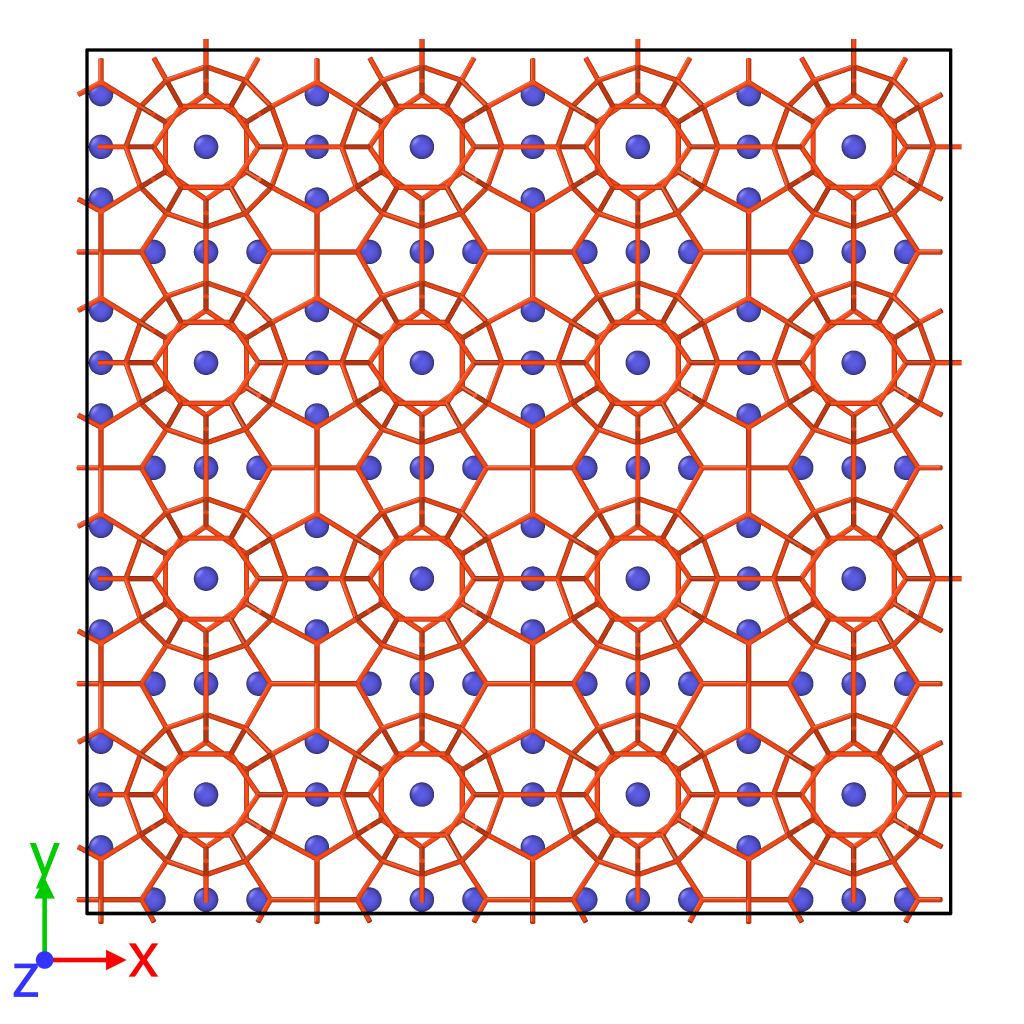
\includegraphics[width=.5\linewidth]{figures/unit3a.png}
    \end{minipage}
    \caption{Топология водородных связей в исходной ячейке моделирования. Связи показаны оранжевыми линиями, синими шариками -- молекулы метана, молекулы воды не отображены.}
    \label{fig3.2}
\end{figure}

На первом этапе моделирования производилось плавление кристаллической решетки гидрата метана при температуре $T=425$ К и давлении $p=500$ атмосфер до полного исчезновения исходной кристаллической структуры и образования двухфазной жидкой системы метан-вода,. После, данная конфигурация была переохлаждена в нескольких различных симуляциях до температуры $T=210$ К с высокими скоростями охлаждения $\gamma_1=10^{10}$ К/с и $\gamma_2=10^{11}$ К/с, затем наблюдался процесс затвердевания данной системы и образования гидрата метана в течение 50 нс.

\begin{figure}[H]
    \centering
    \begin{minipage}{\linewidth}
        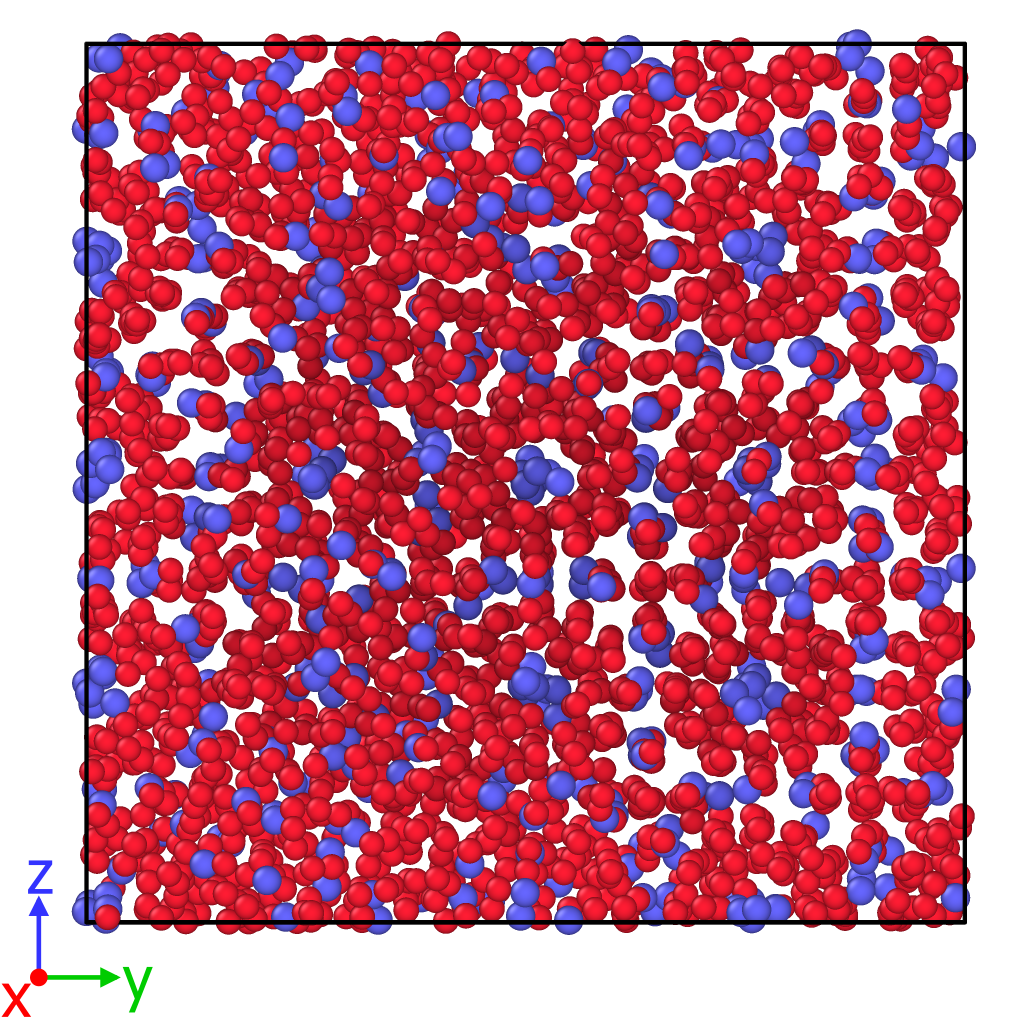
\includegraphics[width=.49\linewidth]{figures/press1.png}\hfill
        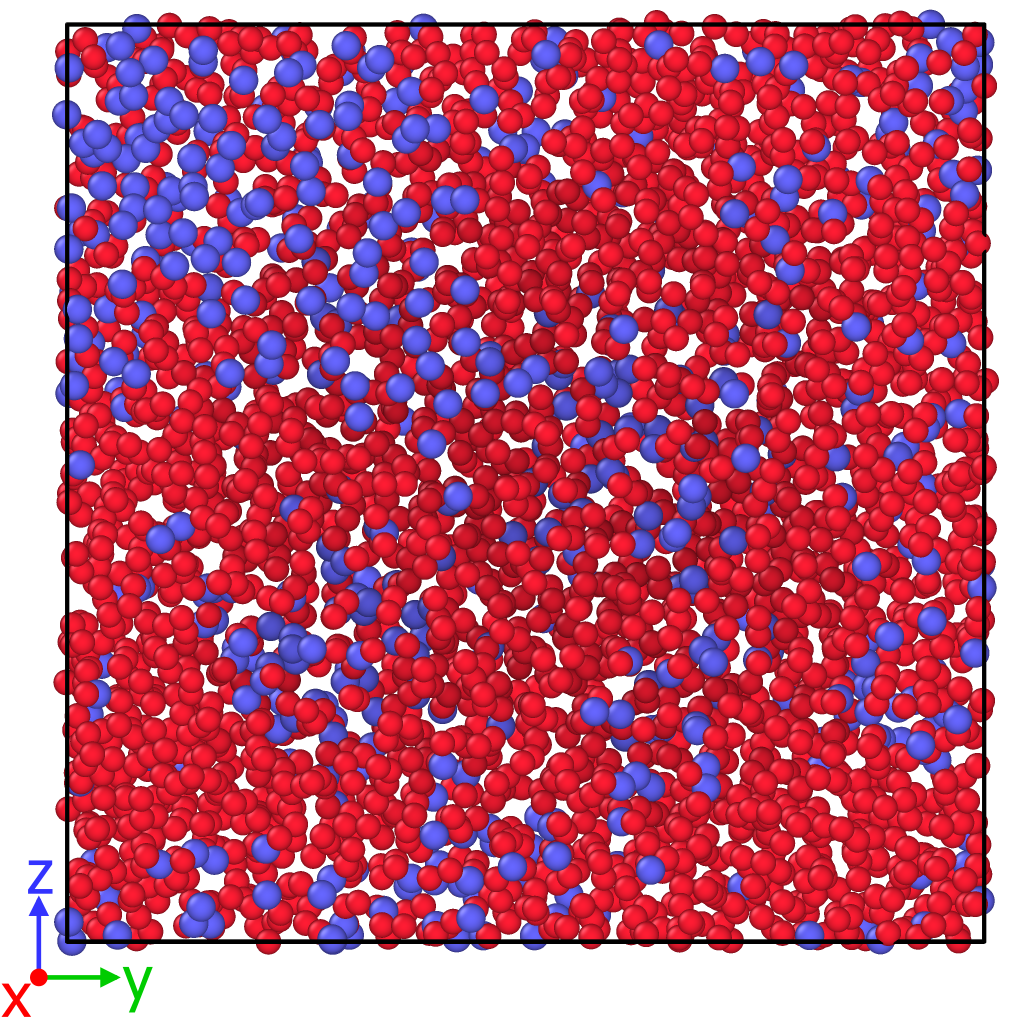
\includegraphics[width=.49\linewidth]{figures/press2.png}
    \end{minipage}
    \begin{minipage}{\linewidth}
        \centering
        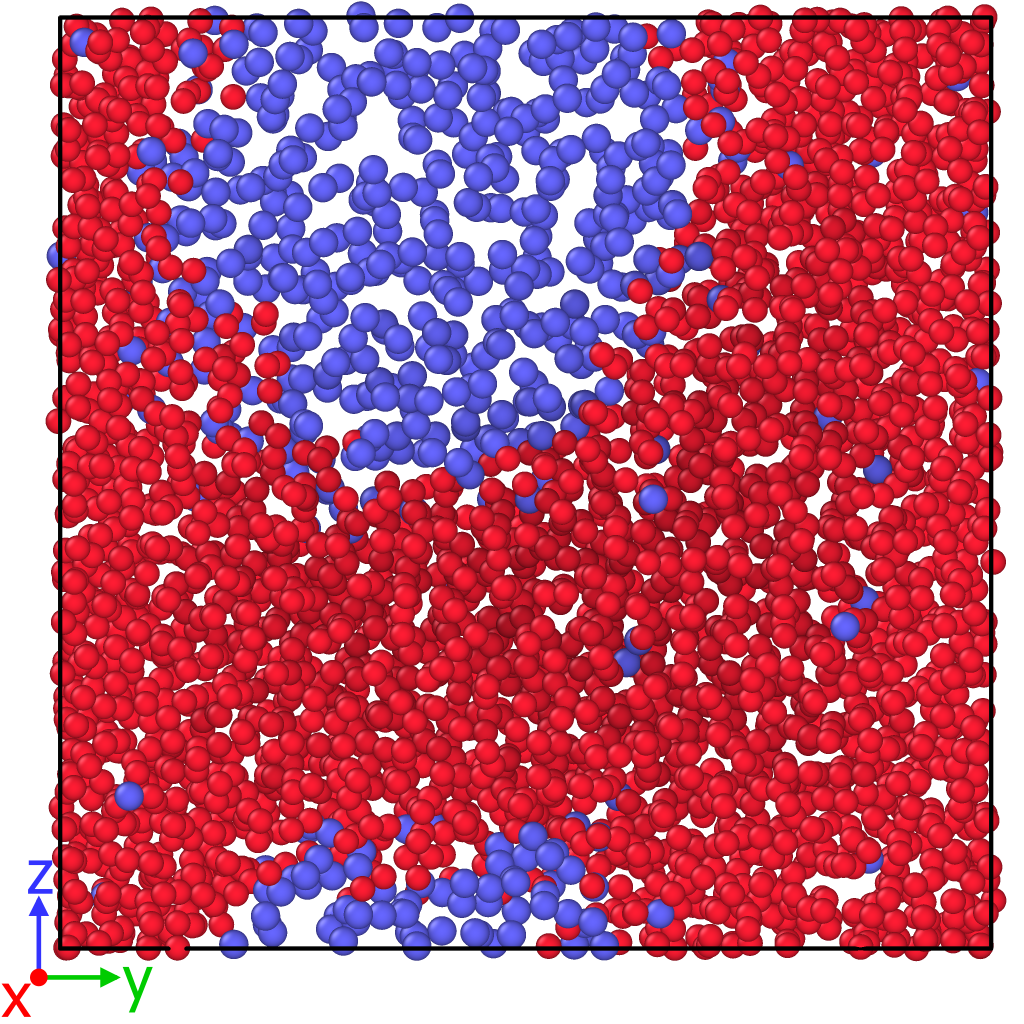
\includegraphics[width=.5\linewidth]{figures/press3.png}
    \end{minipage}
    \caption{Последовательные этапы плавления ячейки моделирования при $T=425$ К и $p=500$ атмосфер.}
    \label{fig3.3}
\end{figure}

\begin{figure}[H]
    \centering
    \begin{minipage}{\linewidth}
    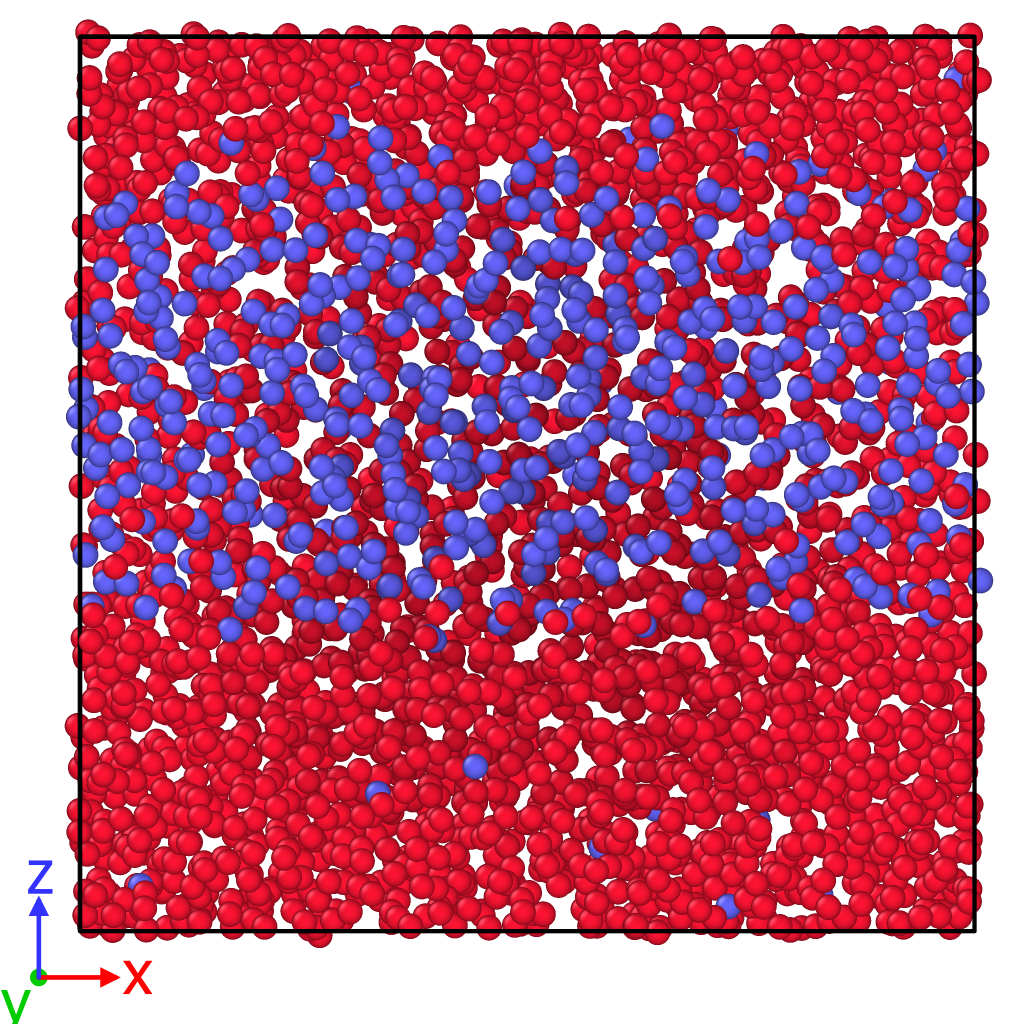
\includegraphics[width=.49\linewidth]{figures/cool1.png}
    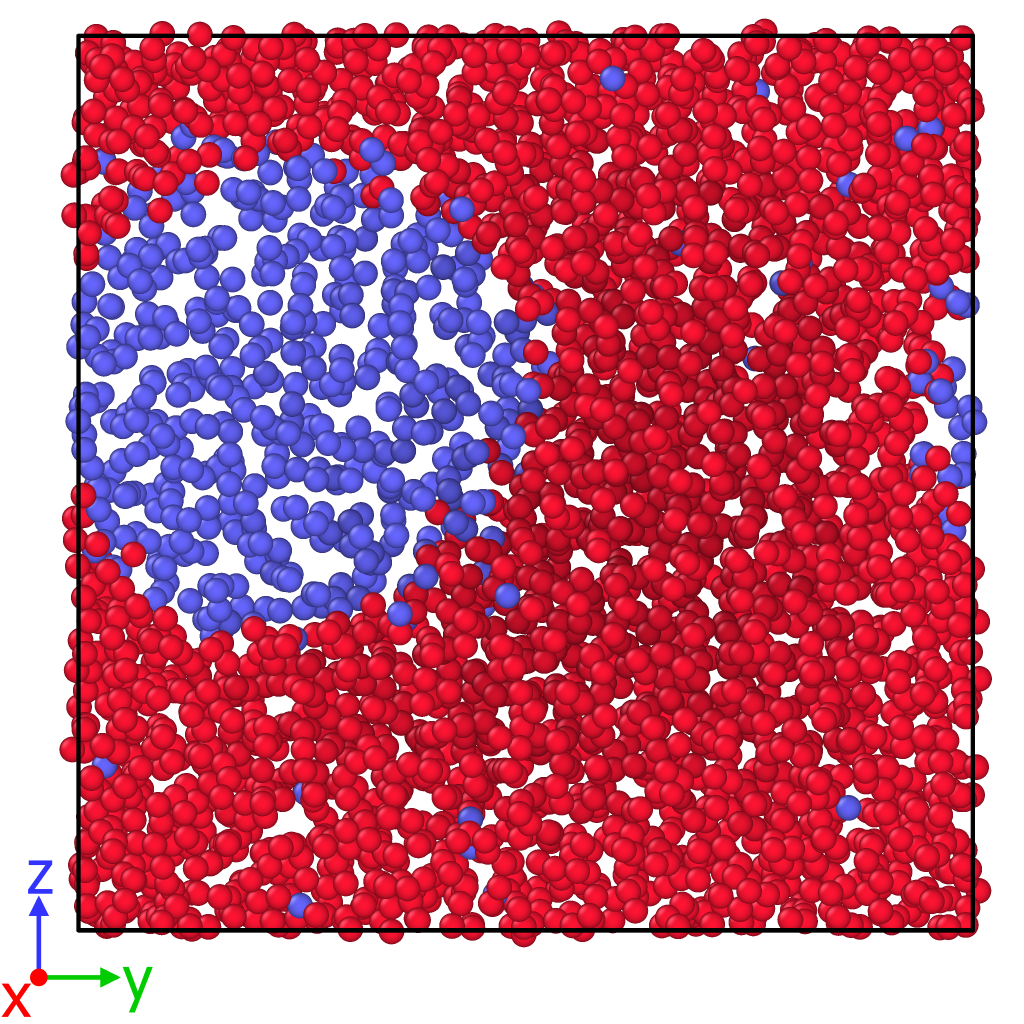
\includegraphics[width=.49\linewidth]{figures/cool2.png}
    \end{minipage}
    \begin{minipage}{\linewidth}
        \centering
        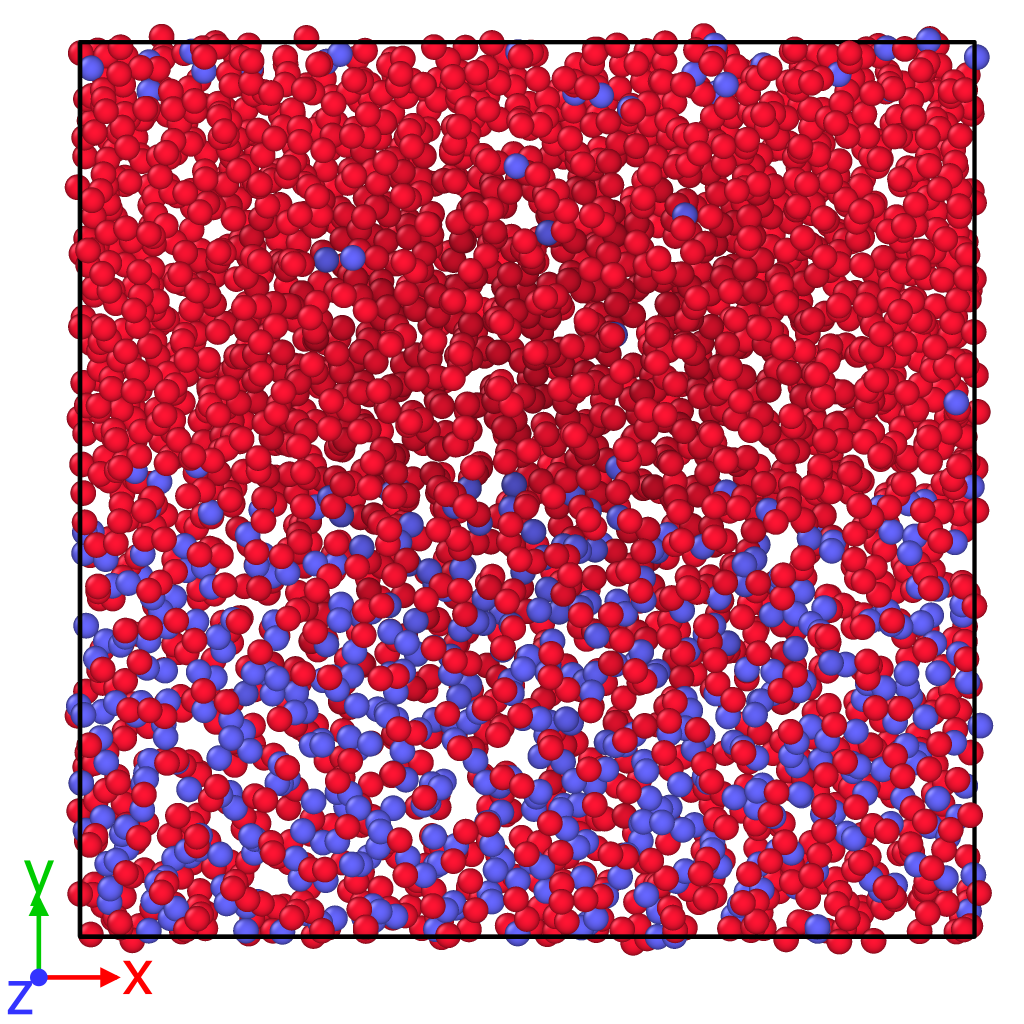
\includegraphics[width=.5\linewidth]{figures/cool3.png}
    \end{minipage}
    \caption{Конфигурация переохлажденной со скоростью $\gamma=10^{11}$ К/с двухфазной жидкости при $T=210$ К и $p=500$.}
    \label{fig3.4}
\end{figure}

Выбор именно этой температуры, соответствующей глубокому переохлаждению гидрата метана, был мотивирован тем, что при данной температуре в более ранних работах авторами используемой модели был достигнут быстрый, практически мгновенный рост фазы гидрата метана в системе. Кроме того, значения используемых параметров взаимодействия метан-вода $\sigma_{wm}=4,05 \si{\angstrom}$ и $\varepsilon_{wm}=0,240$ ккал/моль, несколько отличаются от приведенных нами ранее при обзоре крупнозернистой модели взаимодействия, по примеру тех же авторов. Хотя такие значения $\sigma_{wm}$ и $\varepsilon_{wm}$ дают большие значения величины растворимости метана в воде (0,0038 против 0,0022) и температуры плавления гидрата метана (301 К против 286 К) , структурные характеристики, в частности, радиальная функция распределения метан-вода, практически одинаковы в обоих случаях.

Принимая во внимание статистическую природу процесса нуклеации гидрата метана, для каждой из скоростей охлаждения было проведено моделирование роста гидрата метана для 10 идентичных систем. На рис. \ref{fig3.5}-\ref{fig3.6} приведены снимки системы в различные моменты времени, отражающие эволюцию системы. Образование зародыша критического размера происходит на границе раздела фаз вода-метан, после чего происходит быстрый рост гидрата метана, причем полного растворения газа не происходит, что объясняется нестехиометричностью гидратов.

\begin{figure}[H]
    \centering
    \begin{minipage}{\linewidth}
        \centering
        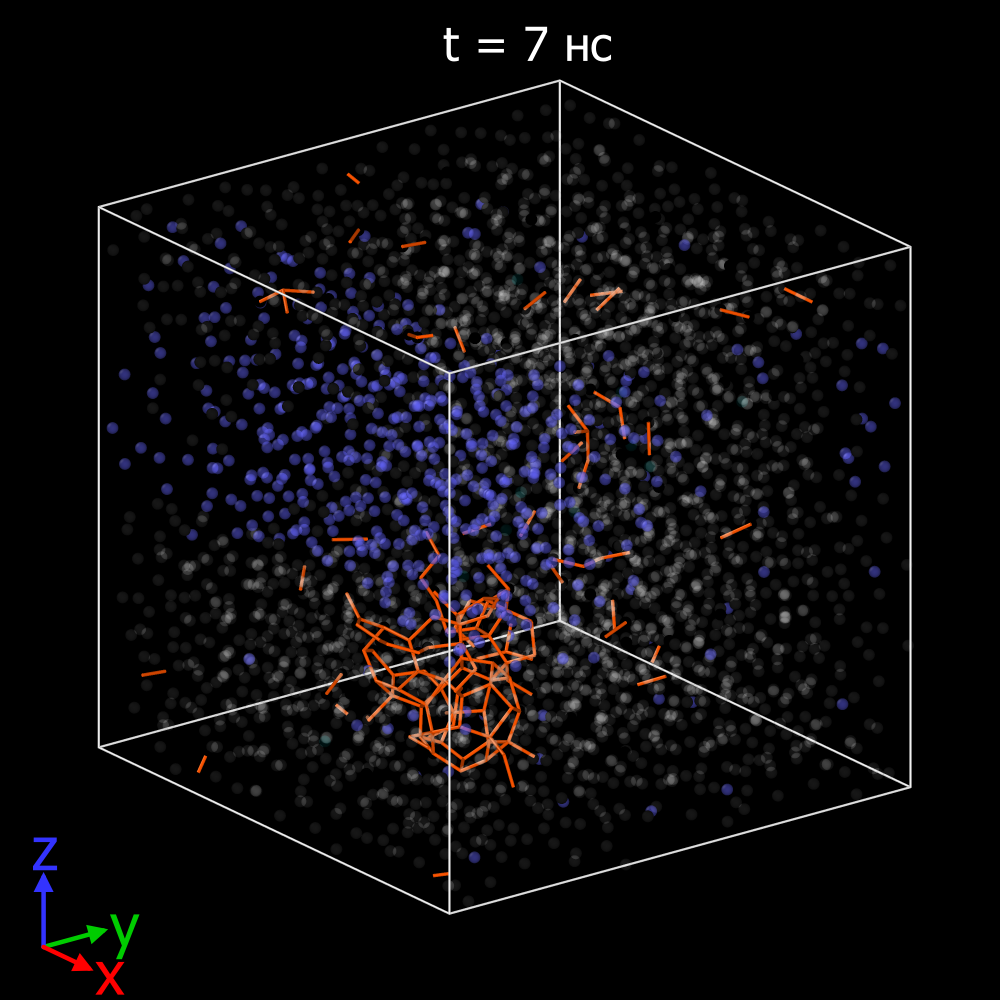
\includegraphics[width=.4\linewidth]{figures/nuclei7.png}
        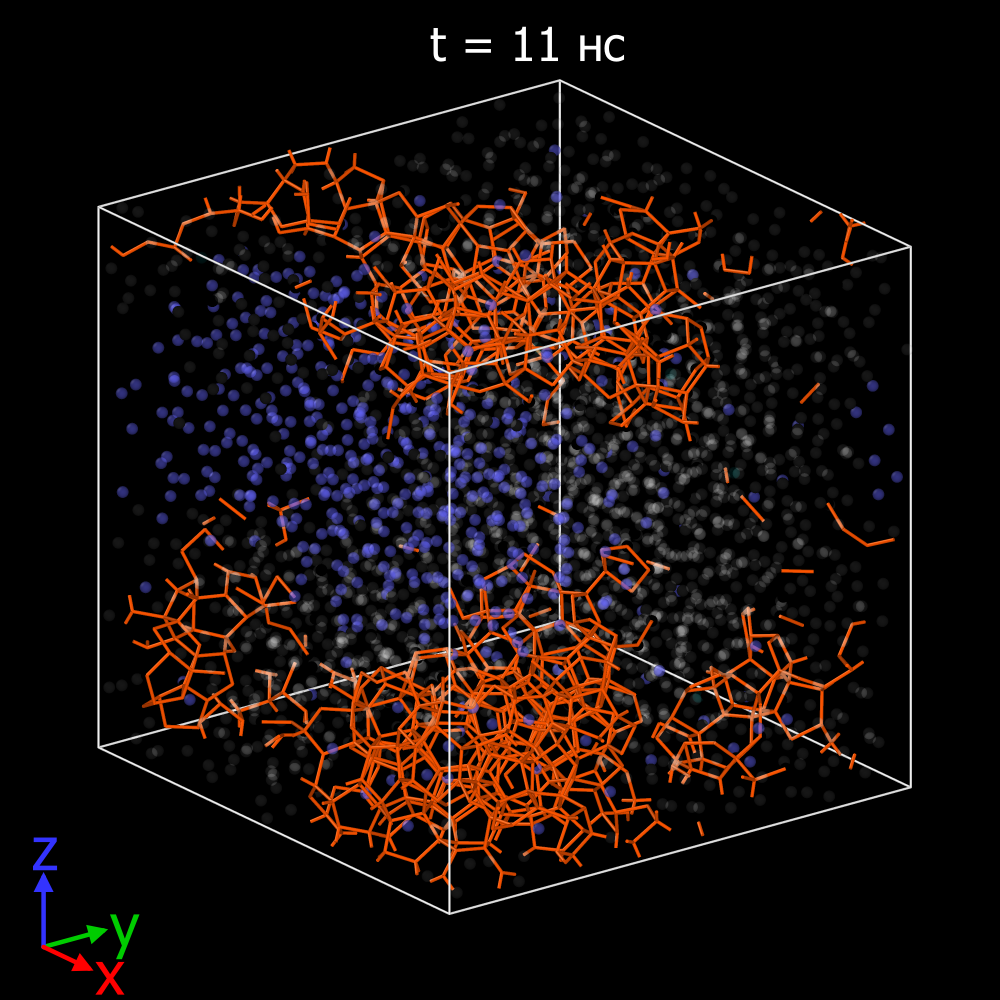
\includegraphics[width=.4\linewidth]{figures/nuclei8.png}
    \end{minipage}
    \begin{minipage}{\linewidth}
        \centering
        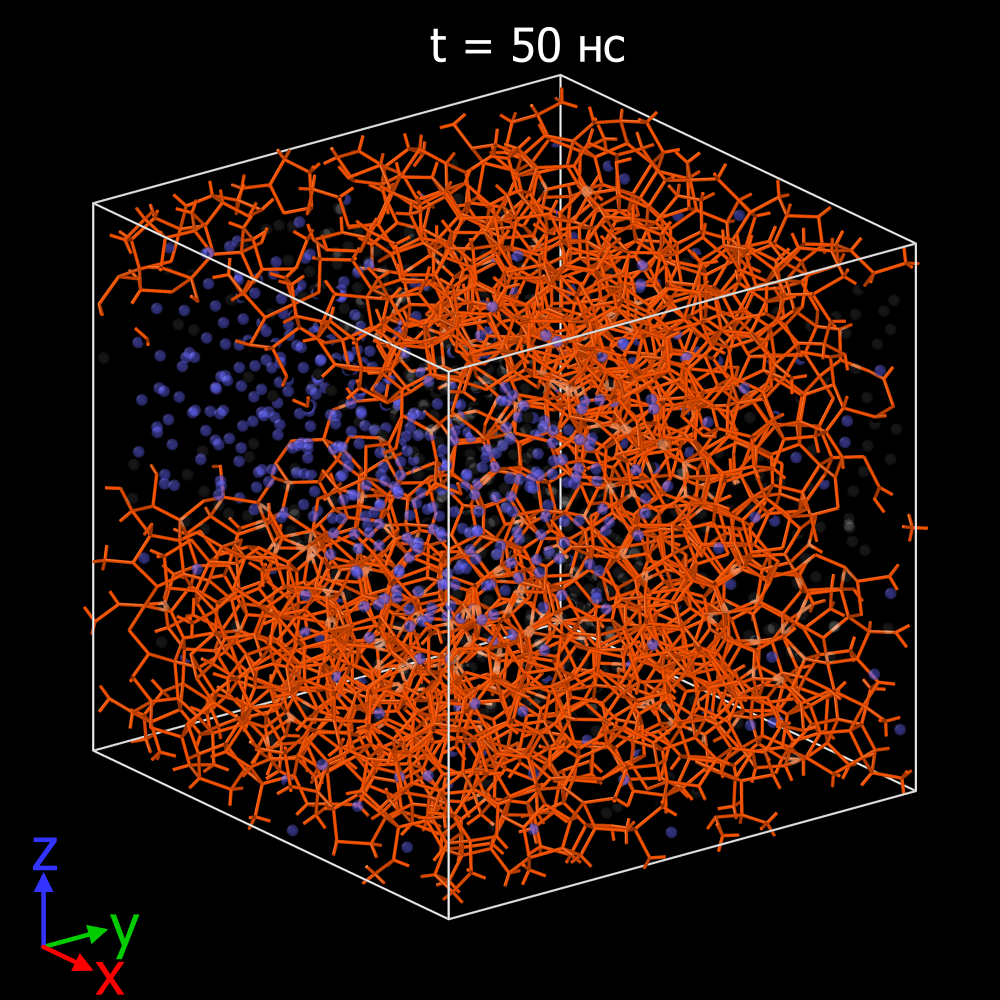
\includegraphics[width=.4\linewidth]{figures/nuclei9.png}
    \end{minipage}
    \caption{Зародышееообразование и рост гидрата метана из переохлажденной со скоростью $\gamma=10^{11}$ К/с двухфазной жидкости при $T=210$ К и $p=500$ атмосфер. Трехмерная проекция.}
    \label{fig3.6}
\end{figure}

\begin{figure}[H]
    \centering
    \begin{minipage}{\linewidth}
        \centering
        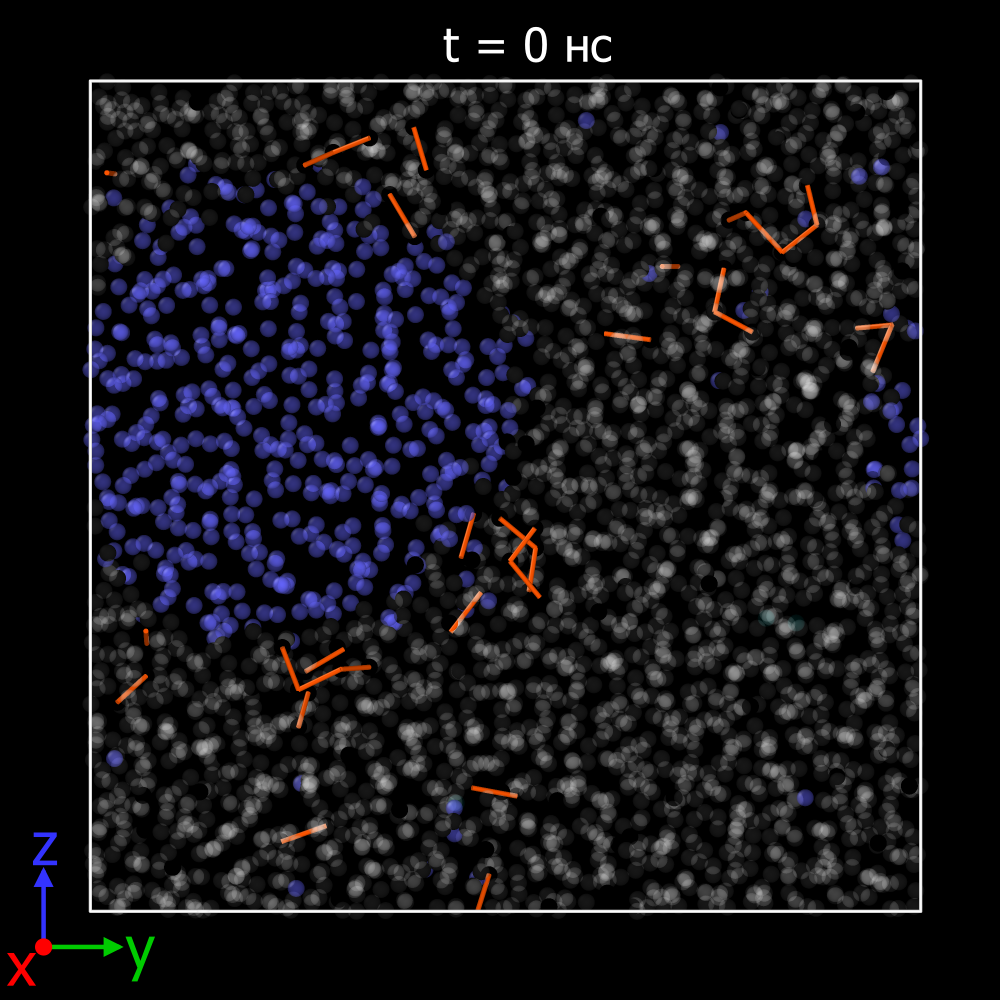
\includegraphics[width=.4\linewidth]{figures/nuclei1.png}
        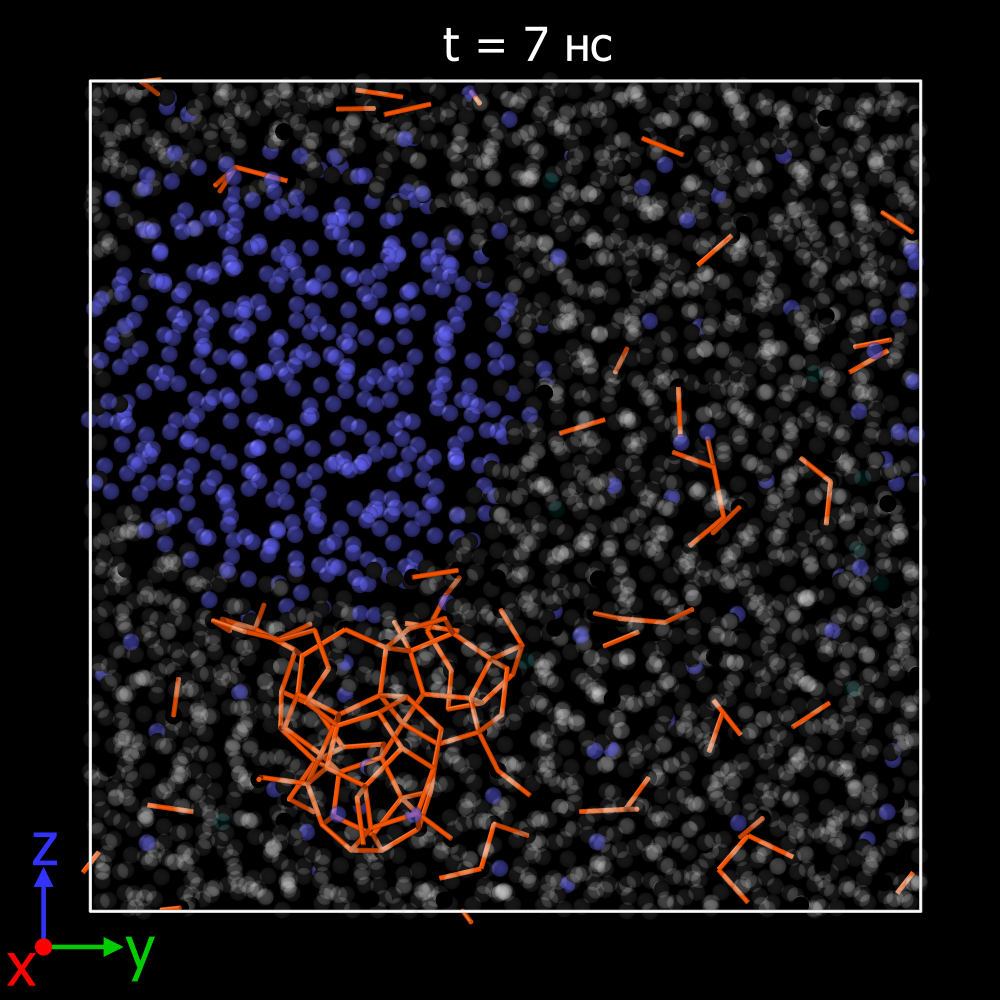
\includegraphics[width=.4\linewidth]{figures/nuclei2.png}
    \end{minipage}\vfill
    \begin{minipage}{\linewidth}
        \centering
        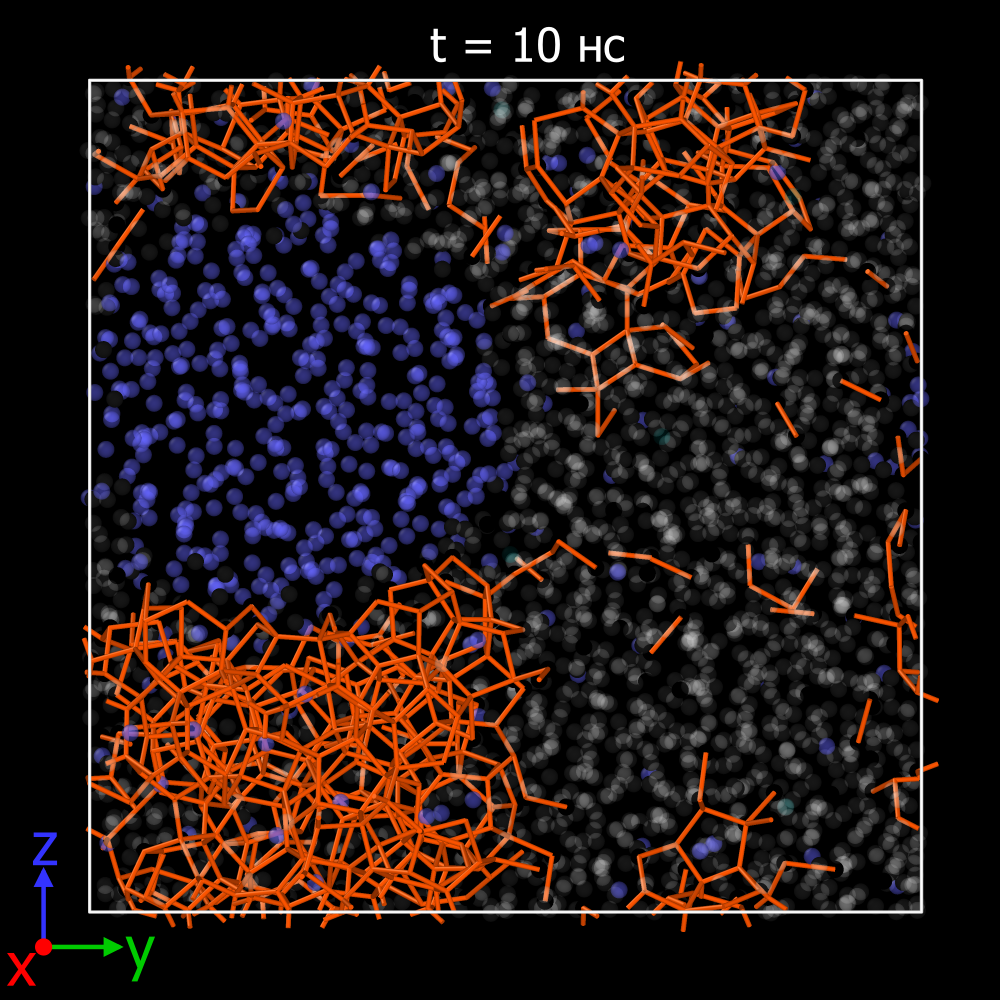
\includegraphics[width=.4\linewidth]{figures/nuclei3.png}
        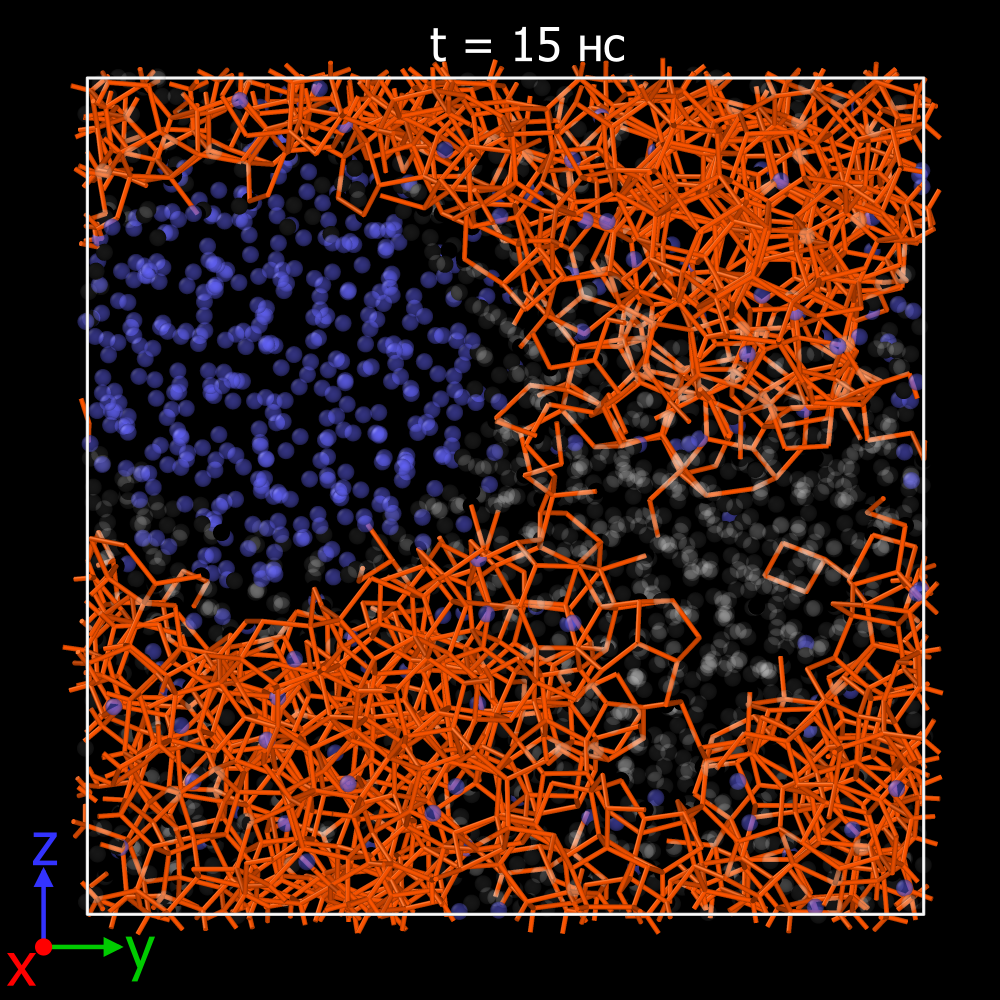
\includegraphics[width=.4\linewidth]{figures/nuclei4.png}
    \end{minipage}\vfill
    \begin{minipage}{\linewidth}
        \centering
        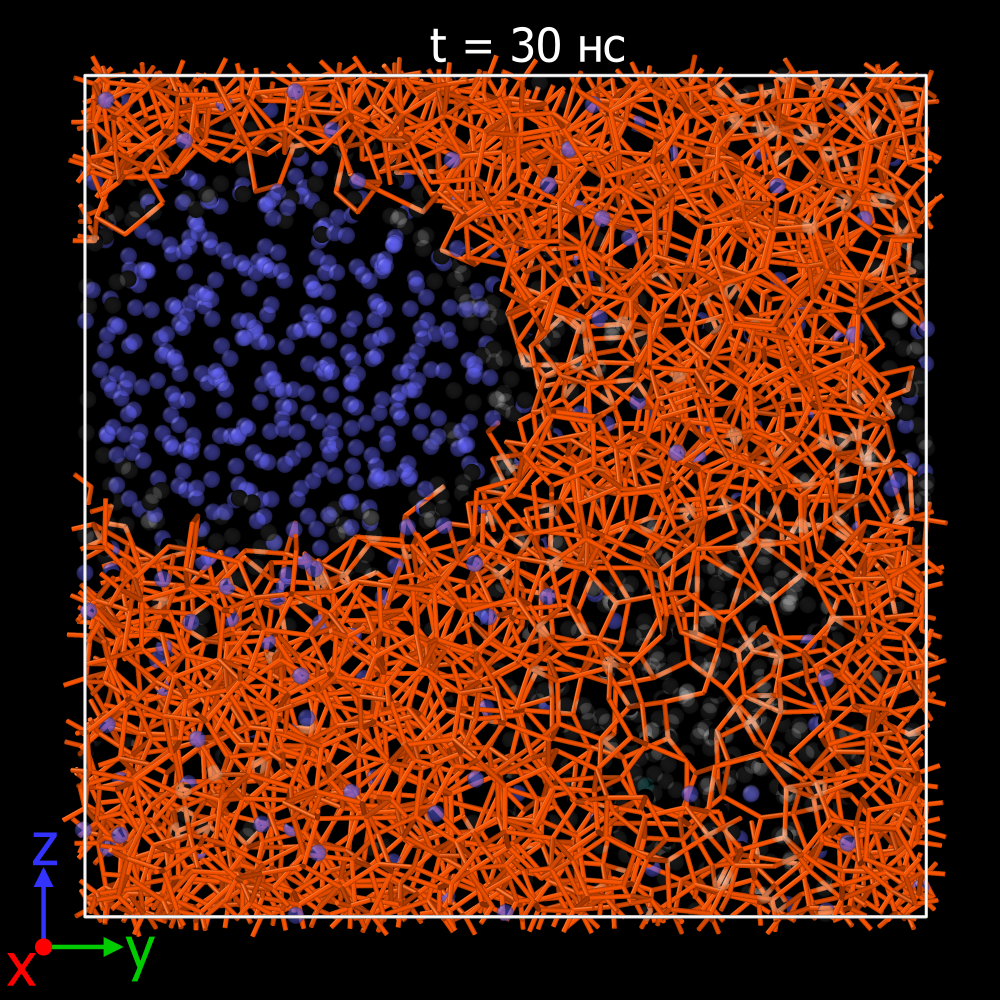
\includegraphics[width=.4\linewidth]{figures/nuclei5.png}
        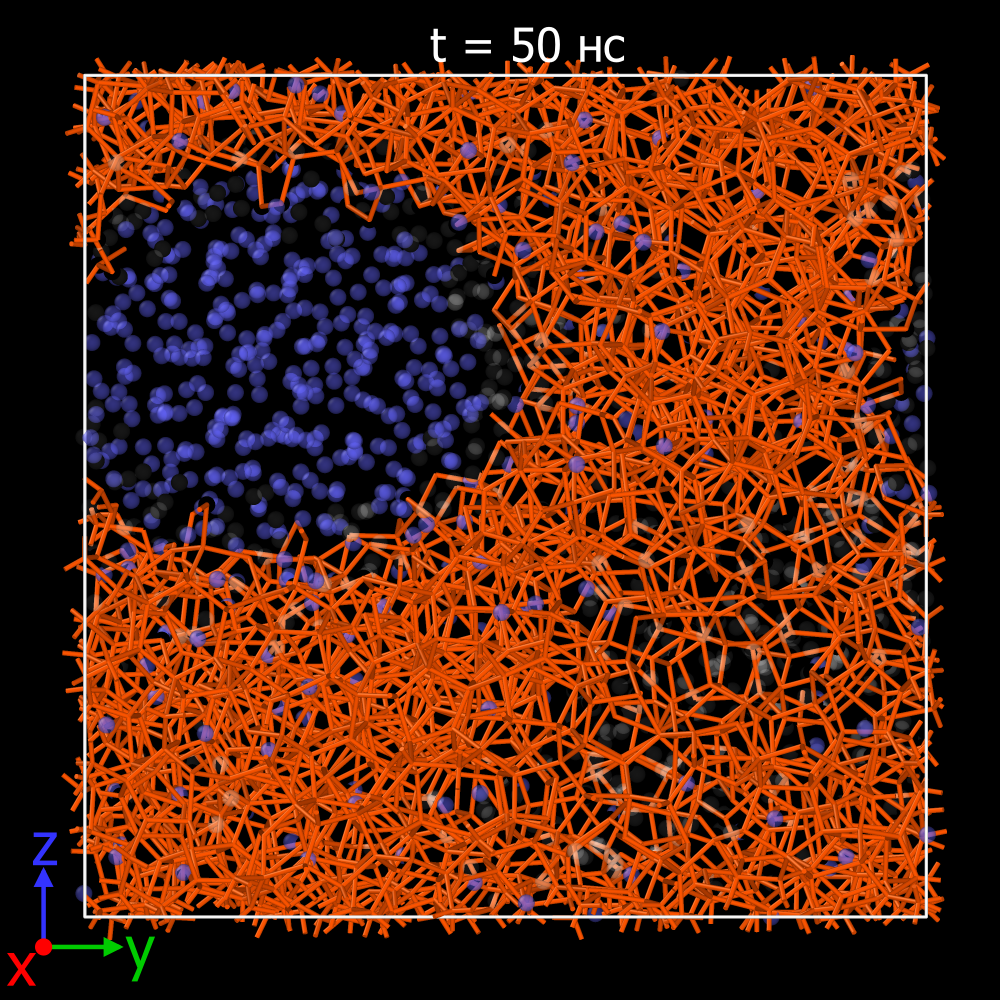
\includegraphics[width=.4\linewidth]{figures/nuclei6.png}
    \end{minipage}
    \caption{Зародышееообразование и рост гидрата метана из переохлажденной со скоростью $\gamma=10^{11}$ К/с двухфазной жидкости при $T=210$ К и $p=500$. Фаза гидрата была идентфицирована при помощи алгоритма CHILL+, соответствующие водородные связи отрисованы оранжевым цветом. Синие шарики -- молекулы метана, белые шарики -- молекулы воды, не находящиеся в фазе гидрата.}
    \label{fig3.5}
\end{figure}

После чего были построены зависимости содержания фазы гидрата от времени моделирования с использованием алгоритма CHILL+.

\begin{figure}[H]
    \centering
    \begin{minipage}{\linewidth}
        \centering
        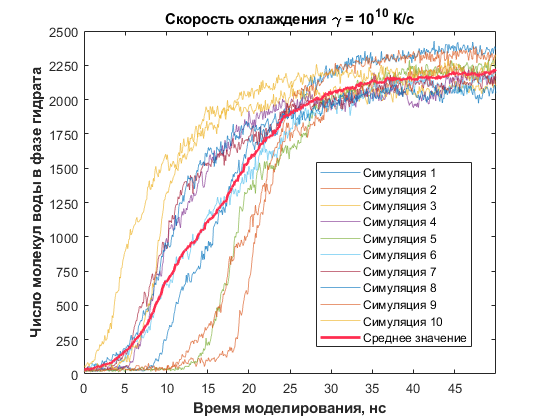
\includegraphics[width=.7\linewidth]{figures/bulk10.png}
    \end{minipage}
    \begin{minipage}{\linewidth}
        \centering
        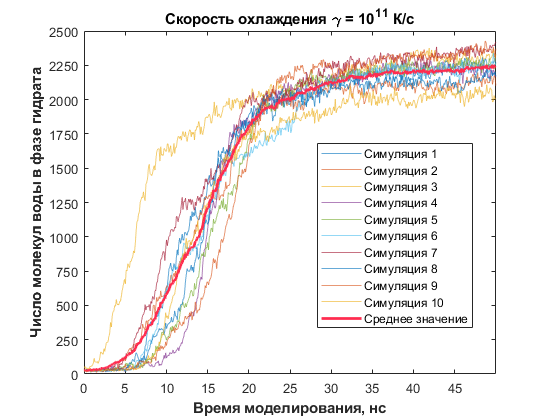
\includegraphics[width=.7\linewidth]{figures/bulk11.png}
    \end{minipage}
    \caption{Зависимости числа молекул воды, образующих структуру гидрата, от времени моделирования при различных скоростях моделирования. Температура $T=210$ К, давление $p=500$ атмосфер.}
    \label{fig3.7}
\end{figure}

Из анализа и сравнения полученных зависимостей рис. \ref{fig3.7}-\ref{fig3.8} следуют несколько выводов:
\begin{enumerate}
    \item На большой части зависимости рост фазы гидрата происходит приблизительно по линейной зависимости, независимо от скорости охлаждения образца.
    \item При более высокой скорости переохлаждения наклон этой линейной зависимости становится круче, и рост гидратов, соответственно, происходит быстрее.
    \item При скорости охлаждения $10^{11}$ К/с стадия роста для всех, за исключением одной, произведенных симуляций начинается практически одновременно, зародышеообразование просходит в момент времени около 5 нс. В случае скорости охлаждения $\gamma=10^10$ К/с, моменты времени, соответствующие возникновению зародыша критического размера, разнесены друг от друга значительно.
\end{enumerate}

\begin{figure}[H]
    \centering
    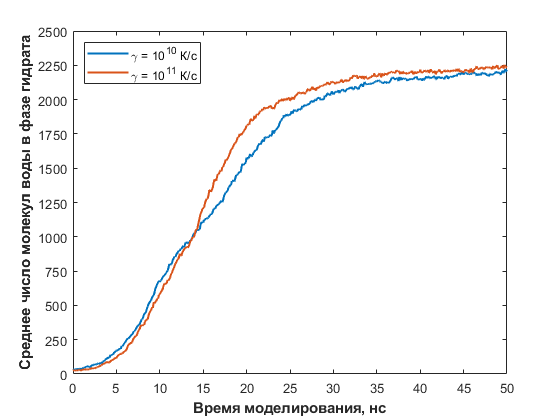
\includegraphics[width=.9\linewidth]{figures/bulk.png}
    \caption{Число молекул в фазе гидрата при $T=210$ К, усредненное по результатам 10 моделирований для каждой из скоростей охлаждения.}
    \label{fig3.8}
\end{figure}
\pagebreak

\section{Диссоциация гидрата метана в рамках модели TIP4P}
\begin{figure}[H]
    \centering
    \begin{minipage}{\linewidth}
        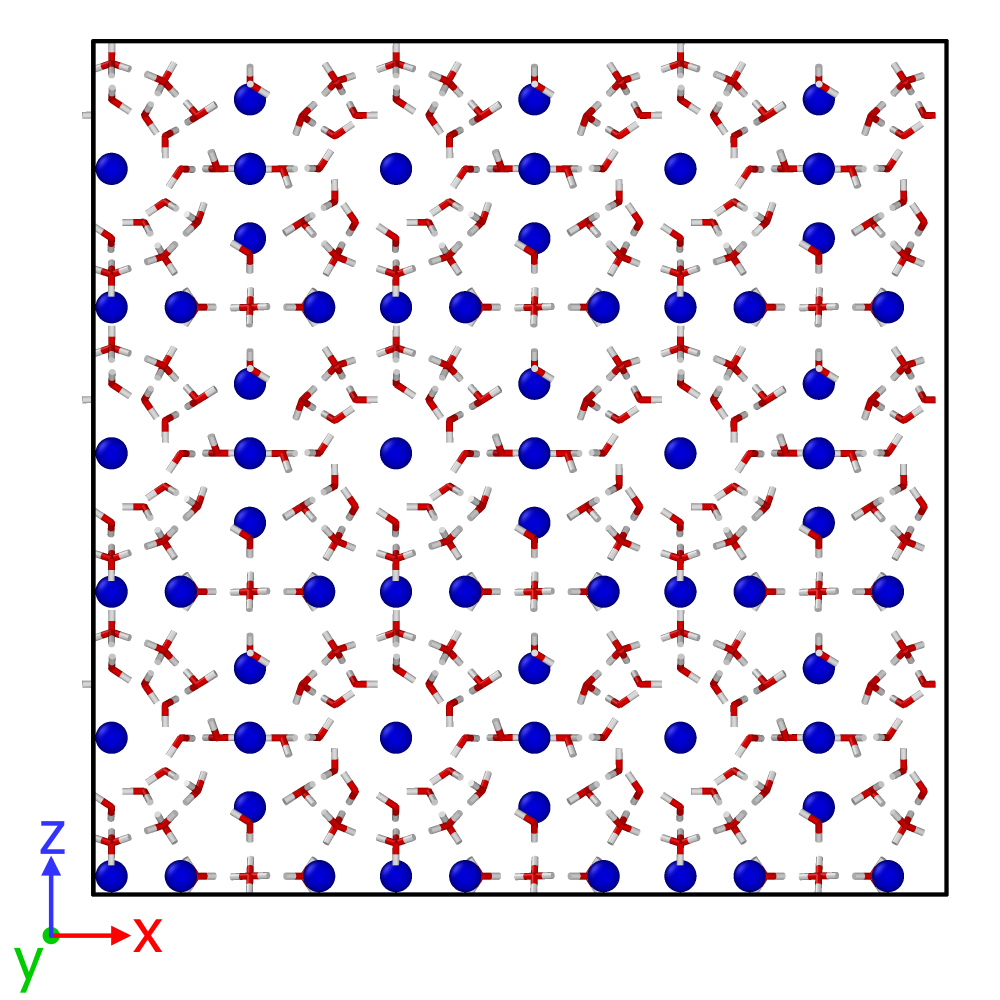
\includegraphics[width=.49\linewidth]{figures/tip4p_unit2.png}
        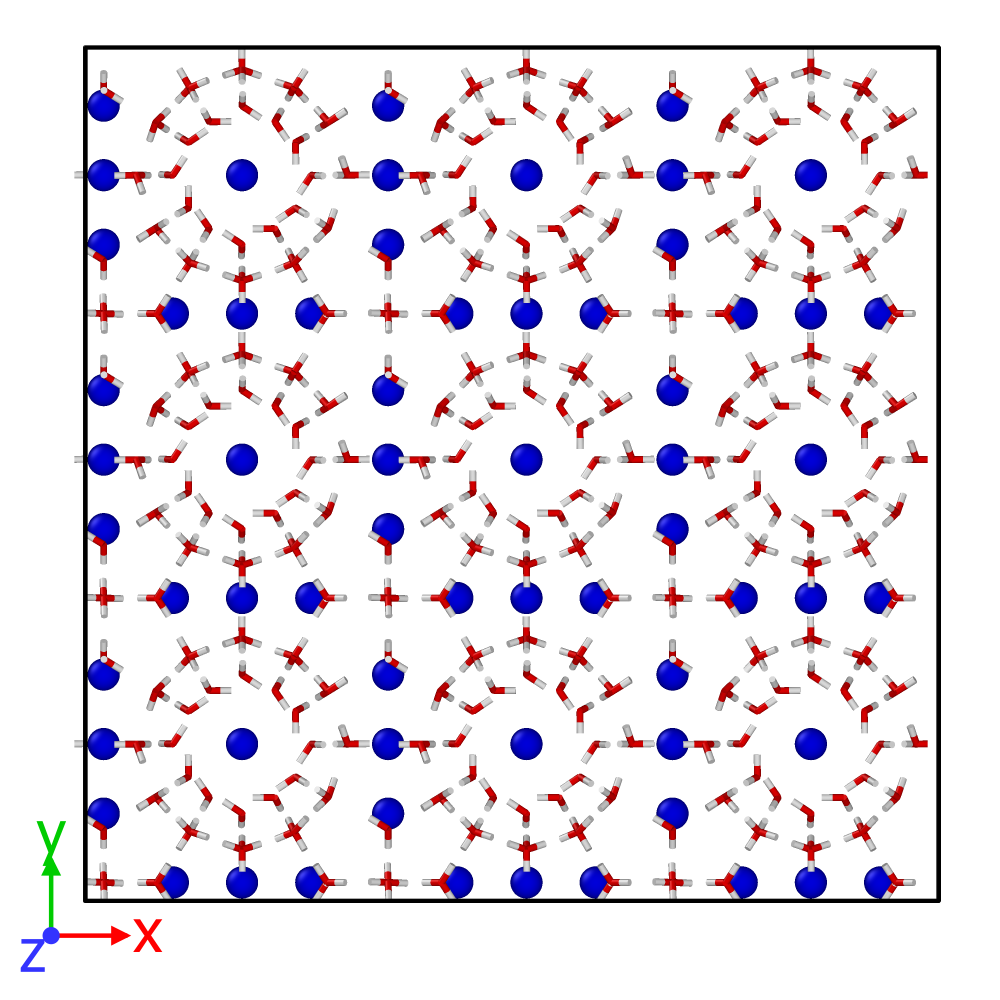
\includegraphics[width=.49\linewidth]{figures/tip4p_unit3.png}
    \end{minipage}
    \begin{minipage}{\linewidth}
        \centering
        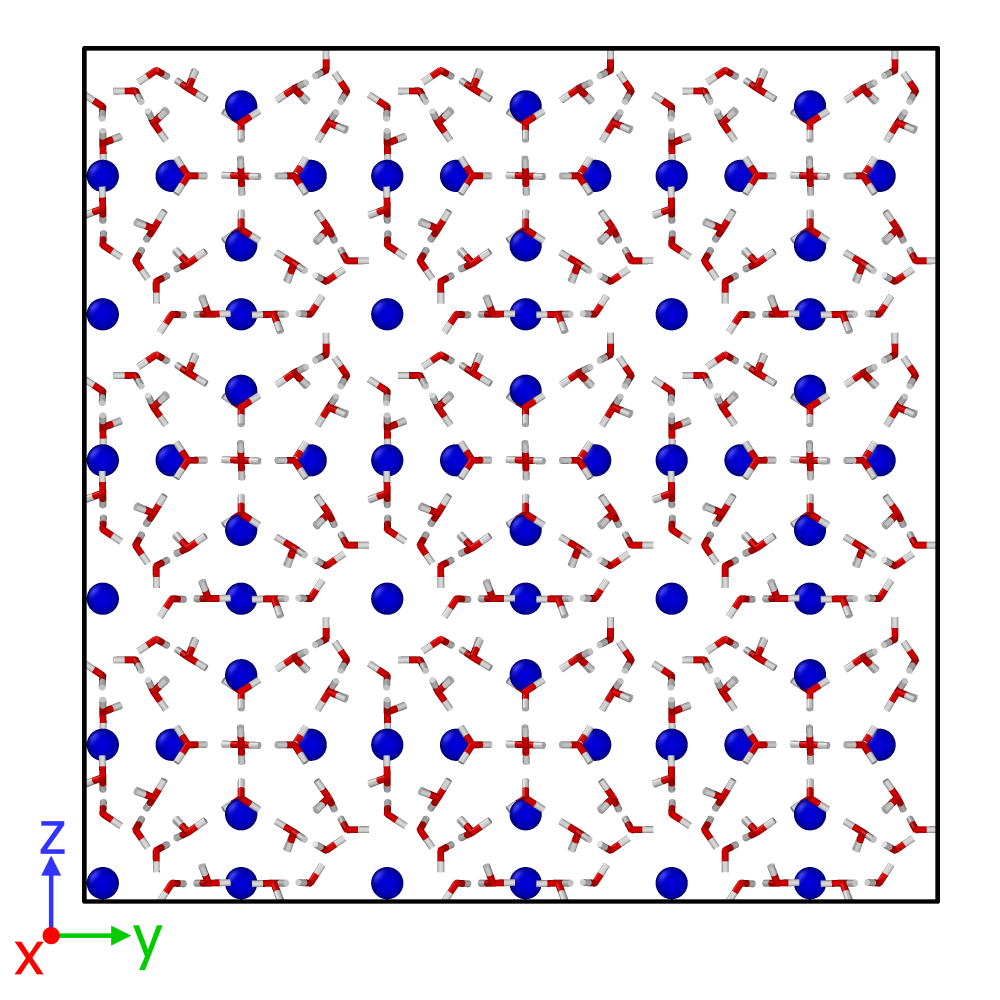
\includegraphics[width=.49\linewidth]{figures/tip4p_unit4.png}
    \end{minipage}
    \caption{Начальная конфигурация системы в различных проекциях. Молекулы воды изображены v-образными палочками, молекулы метана -- синими шариками.}
    \label{fig3.9}
\end{figure}

Был рассмотрен процесс диссоциации $sI$-гидрата метана при давлении $100$ атмосфер и нагреве с $250$ К до $450$ К в течение 10 наносекунд. Исходная система состояла из $3\times 3\times 3\times=27$ элементарных ячеек $sI$-гидрата метана. Для моделирования воды использовался потенциал взаимодействия TIP4P/Ice, взаимодействие метана осуществлялось по модели OPLS-UA. Для нахождения параметров $\varepsilon$ и $\sigma$ перекрестного взаимодействия между водой и метаном применялись правила Лоренца-Бертло. Система состояла из 1242 атомов кислорода, 2484 атомов водорода и 216 молекул метана. Применялся временной шаг 2 фс. Моделирование проводилось для восьми идентичных независимых систем. Процесс диссоциации наблюдался визуально, путем графического изображения ячейки моделирования, а также отслеживались температура, давление в системе, её плотность и величина потенциальной энергии. 

\begin{figure}[H]
    \centering
    \begin{minipage}{\linewidth}
        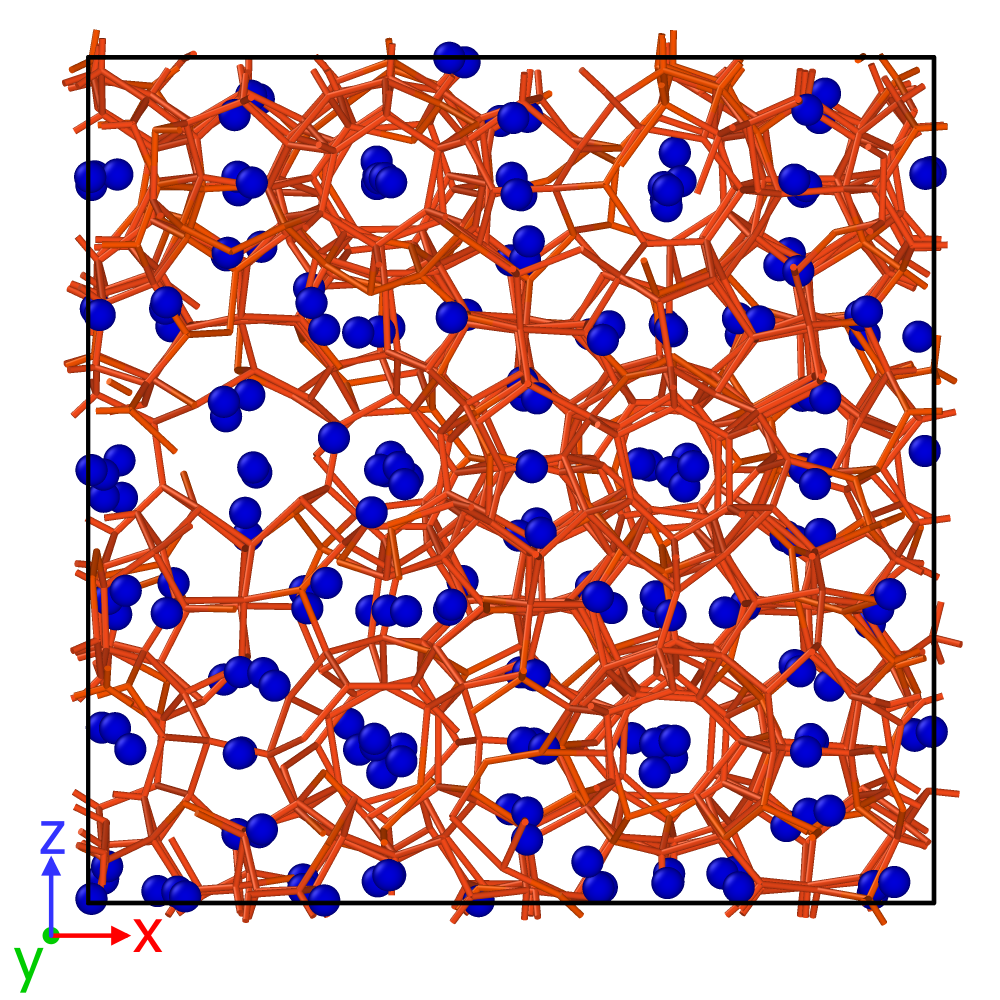
\includegraphics[width=.45\linewidth]{figures/tip4p_melt1.png}
        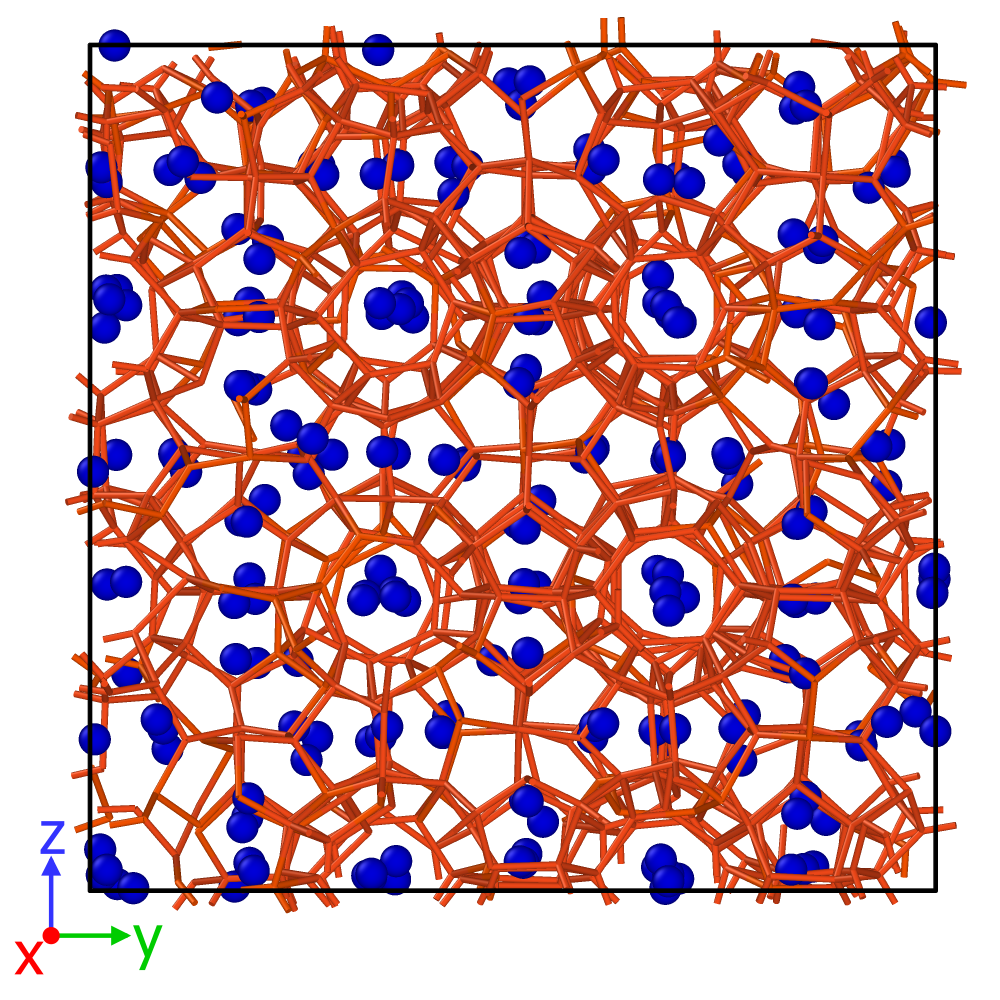
\includegraphics[width=.45\linewidth]{figures/tip4p_melt2.png}
    \end{minipage}
    \begin{minipage}{\linewidth}
        \centering
        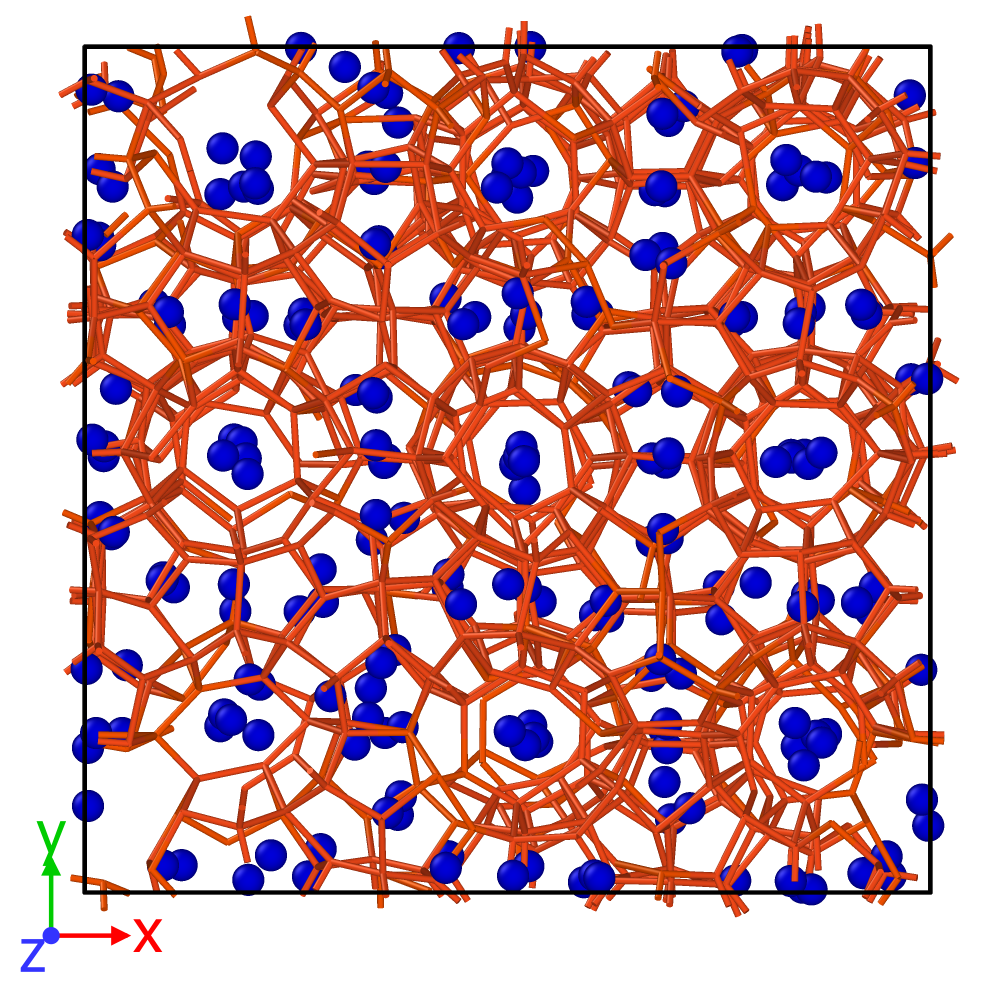
\includegraphics[width=.45\linewidth]{figures/tip4p_melt3.png}
    \end{minipage}
    \caption{Момент начала плавления системы при $T=425$ К в различных проекциях. Связи между молекулами воды в гидрате отрисованы оранжевым цветом. Видны участки, где началось плавление кристалла.}
    \label{fig3.10}
\end{figure}



\begin{figure}[H]
    \centering
    \begin{minipage}{\linewidth}
        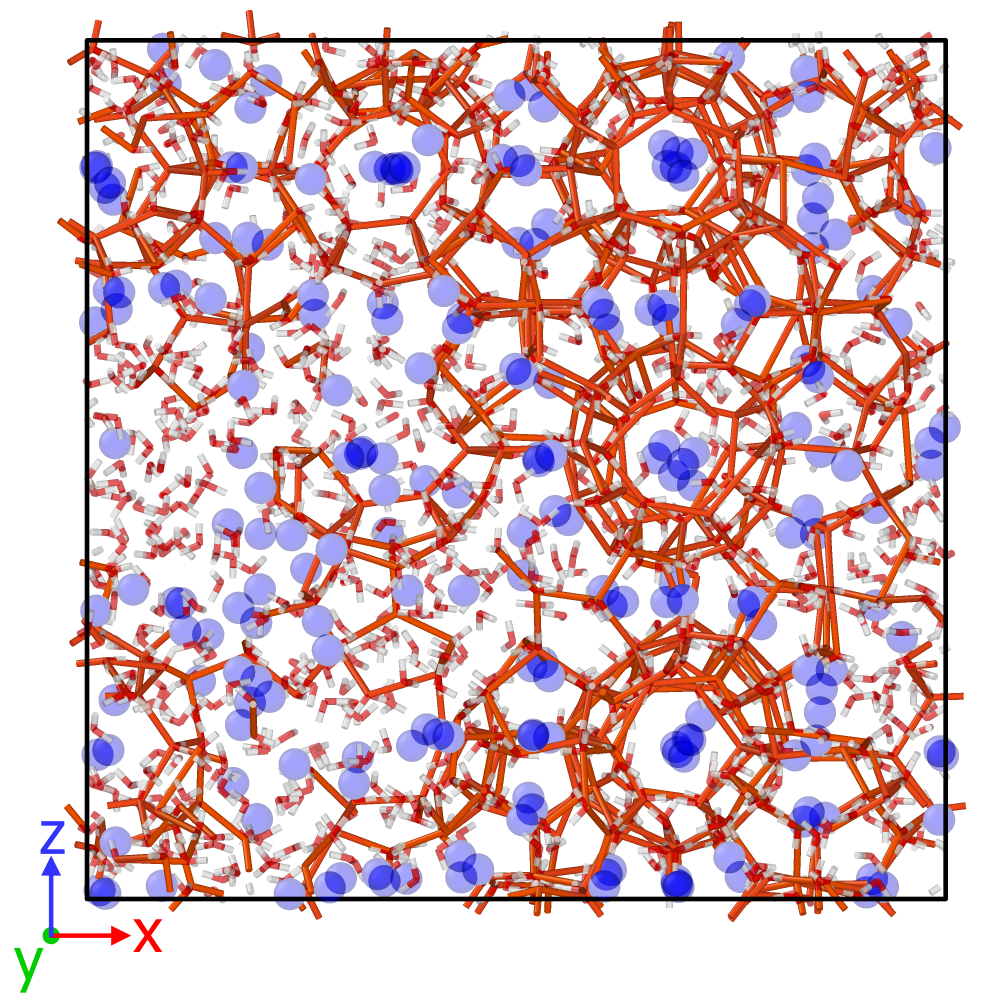
\includegraphics[width=.49\linewidth]{figures/tip4p_melt4.png}
        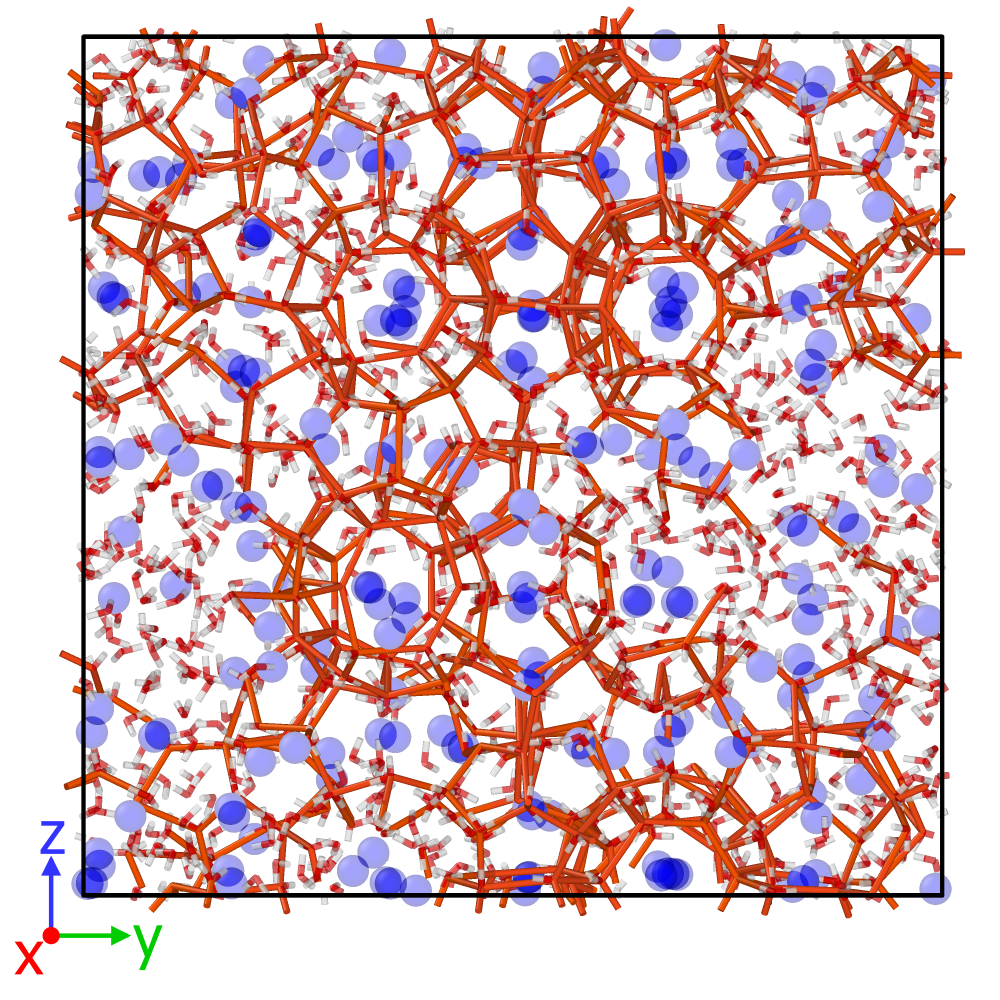
\includegraphics[width=.49\linewidth]{figures/tip4p_melt5.png}
    \end{minipage}
    \begin{minipage}{\linewidth}
        \centering
        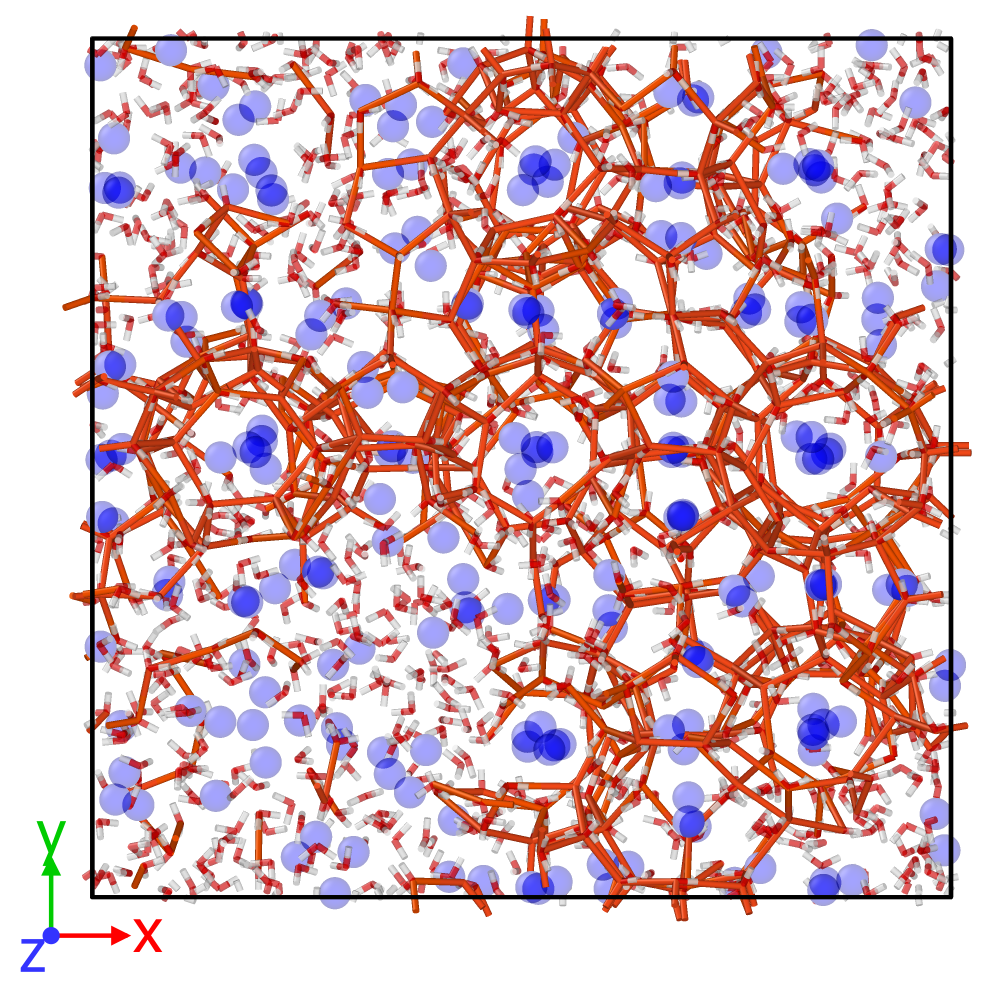
\includegraphics[width=.5\linewidth]{figures/tip4p_melt6.png}
    \end{minipage}
    \caption{Дальнейшее разрушение структуры гидрата.}
    \label{fig3.11}
\end{figure}

\begin{figure}[H]
    \centering
    \begin{minipage}{\linewidth}
        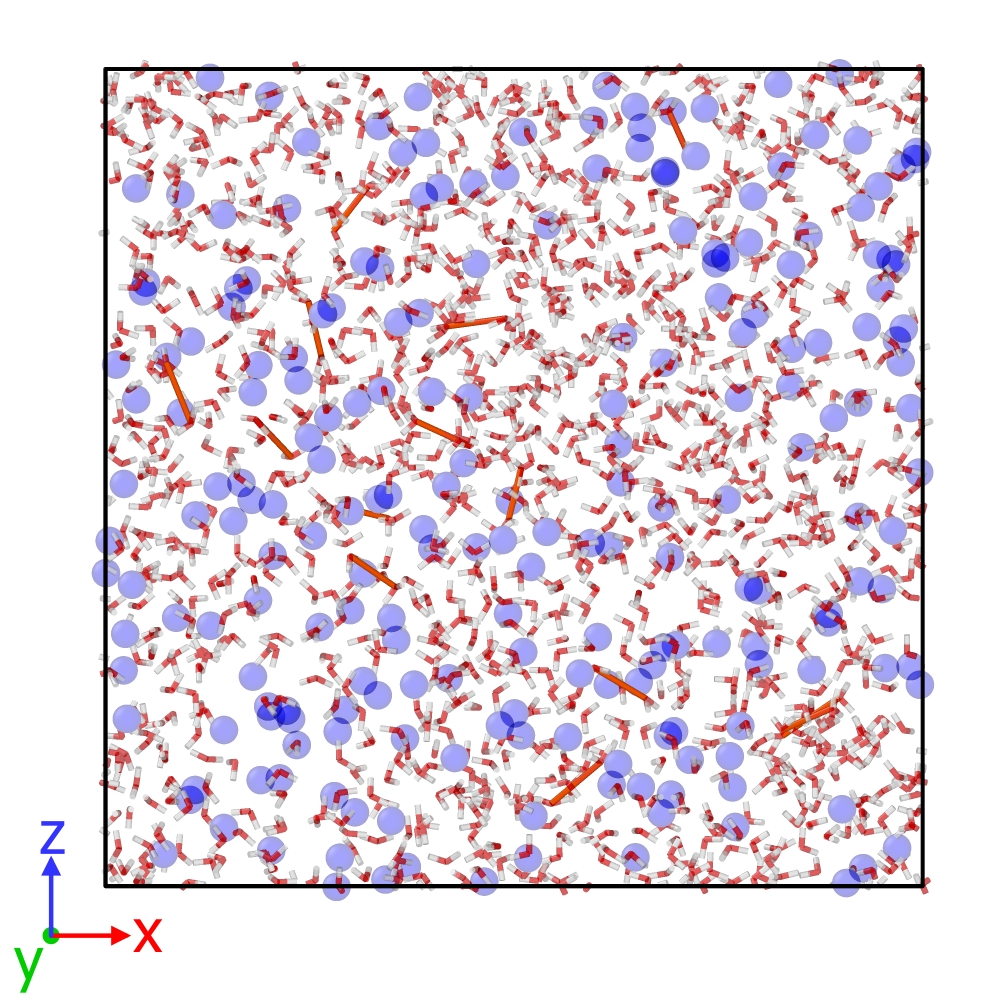
\includegraphics[width=.5\linewidth]{figures/tip4p_melt7.png}\hfill
        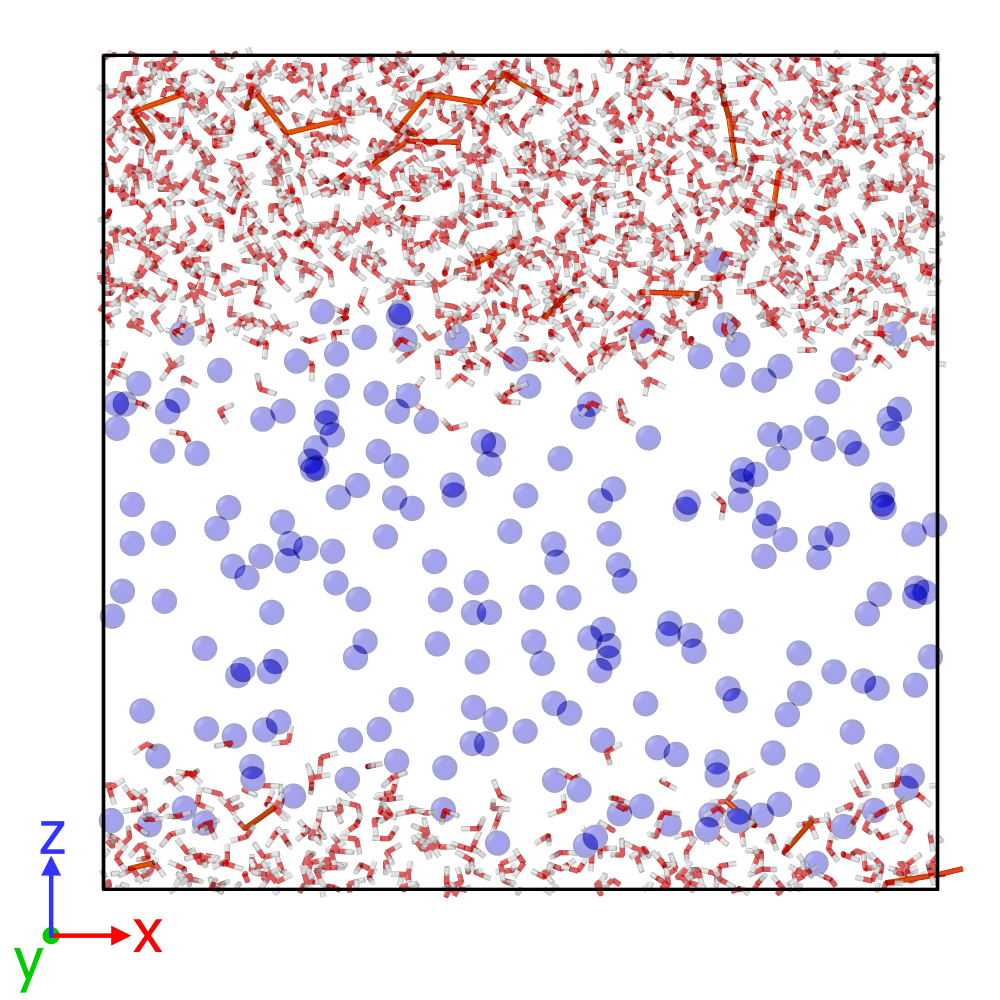
\includegraphics[width=.5\linewidth]{figures/tip4p_melt8.png}
    \end{minipage}
    \caption{Окончательное разрушение структуры гидрата и формирование жидкой двухфазной системы метан-вода.}
    \label{fig3.12}
\end{figure}

Плавлению кристалла гидрата метана, предшествует достаточно длительный промежуток времени, где происходит линейный рост приведенных на рис. \ref{fig3.13} термодинамических характеристик системы. Затем, спустя около 9 нс с начала симуляции, что соответствует температуре системы 425 К, происходит разрыв водородных связей в отдельных полостях решетки (рис. \ref{fig3.10}) и практически мгновенно происходит разрушение структуры гидрата, с последующим формированием двухфазной жидкой системы метан-вода (рис. \ref{fig3.11}-\ref{fig3.12}). 

Число молекул воды, образующих структуру гидрата до момента 9 нс монотонно снижается. Фазовому переходу соответствует скачкообразное падение их количества до нуля. Соответствующая зависимость была получена с использованием алгоритма CHILL+ и представлена на рис. \ref{fig3.14}. Отслеживаемые термодинамические характеристики системы также испытывают резкий скачок в данный момент времени. Сравнивая данные параметры для всех моделирований, можно увидеть что процесс протекает одинаково во всех случаях.

\begin{figure}[H]
    \centering
    \begin{minipage}{\linewidth}
        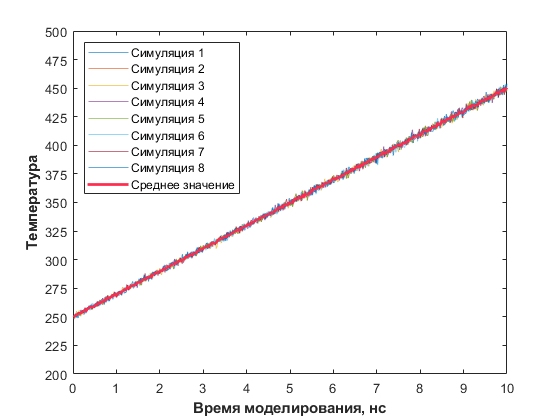
\includegraphics[width=.5\linewidth]{figures/temp.png}\hfill
        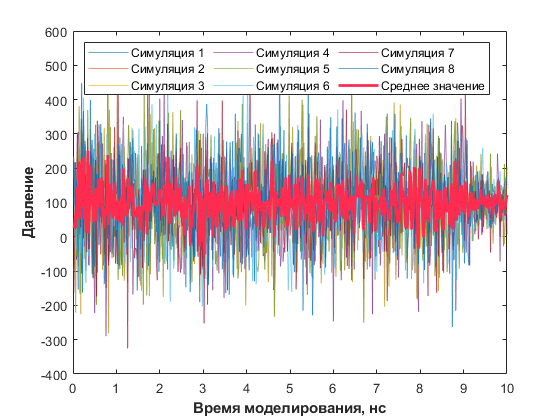
\includegraphics[width=.5\linewidth]{figures/press.png}
    \end{minipage}
    \begin{minipage}{\linewidth}
        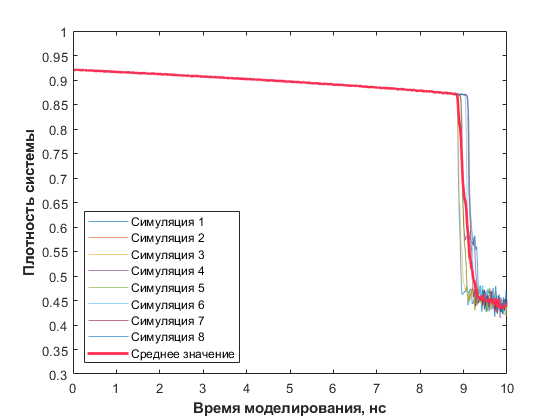
\includegraphics[width=.5\linewidth]{figures/density.png}\hfill
        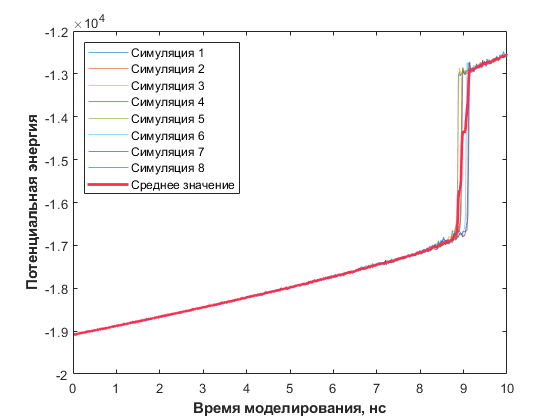
\includegraphics[width=.5\linewidth]{figures/pe.png}
    \end{minipage}
    \begin{minipage}{\linewidth}
        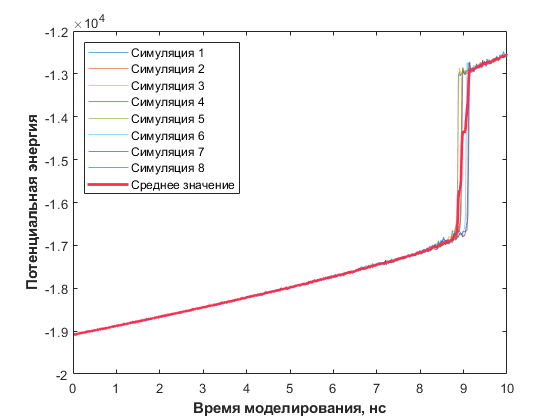
\includegraphics[width=.5\linewidth]{figures/density_temp.png}\hfill
        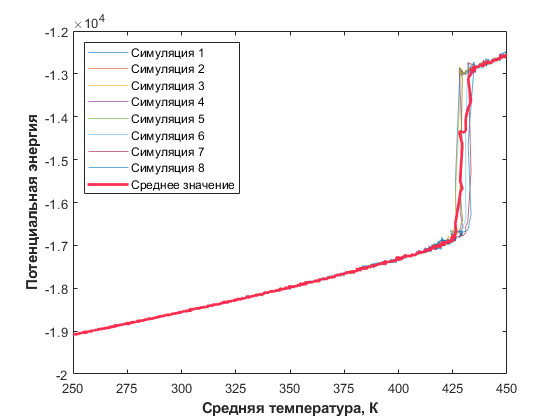
\includegraphics[width=.5\linewidth]{figures/pe_temp.png}
    \end{minipage}
    \caption{Зависимости термодинамических параметров системы: температуры, давления, плотности, потенциальной энергии системы от времени, а также плотности и потенциальной энергии от усредненной температуры.}
    \label{fig3.13}
\end{figure}

\begin{figure}[H]
    \centering
    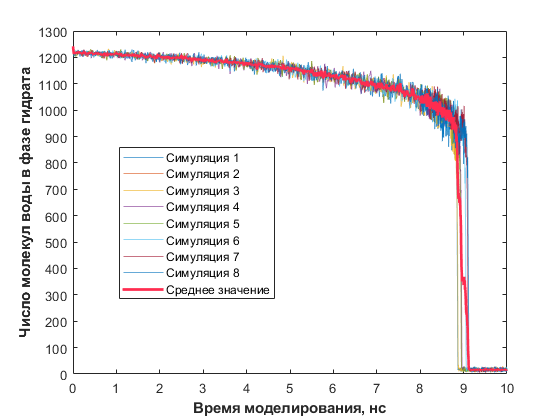
\includegraphics{figures/hydr.png}
    \caption{Зависимость числа молекул воды, составляющих фазу гидрата от времени моделирования.}
    \label{fig3.14}
\end{figure}

Число молекул воды, образующих структуру гидрата до момента 9 нс монотонно снижается. Фазовому переходу соответствует скачкообразное падение их количества до нуля. Соответствующая зависимость была получена с использованием алгоритма CHILL+ и представлена на рис. \ref{fig3.14}. Отслеживаемые термодинамические характеристики системы также испытывают резкий скачок в данный момент времени. Для всех 8 смоделированных систем зависимости температуры, давления, плотности, потенциальной энергии совпадают, и числа молекул воды, принадлежащих фазе гидрата, имеют одинаковый вид.